\documentclass[11pt,twocolumn]{article}
\usepackage{graphicx}
\usepackage[left=1.80cm, right=1.80cm, top=2.00cm, bottom=2.00cm]{geometry}
\usepackage{amsmath,bm}
\usepackage[colorlinks]{hyperref}
\usepackage[natbib=true, sorting=none, backend=biber, bibencoding=utf8, style=ieee]{biblatex}
\usepackage{eurosym}
\usepackage[dvipsnames]{xcolor}
\usepackage{subcaption}
\usepackage{booktabs} % for table (toprule, bottomrule)
\usepackage{enumitem} % for alphabetical enumeration 
\usepackage{accents}
\usepackage{tikz}
\usepackage{dblfloatfix}
\usepackage[printonlyused]{acronym}
\usepackage{cleveref}



\addbibresource{main.bib}
\graphicspath{{../figures/}}

\usetikzlibrary{arrows}
\tikzset{
    vertex/.style={circle,draw,minimum size=1.5em},
    edge/.style={->,> = latex',very thick}
}

\crefname{relation}{Rel.}{Rels.}
\creflabelformat{relation}{(#2#1#3)}
\crefname{constraint}{Constr.}{Constrs.}
\creflabelformat{constraint}{(#2#1#3)}
\crefname{subequations}{Eqs.}{Eqs.}
\creflabelformat{subequations}{(#2#1#3)}

\setlength\parindent{8pt}

% style operators
\newcommand{\ie}{\textit{i.e.} }
\newcommand{\eg}{\textit{e.g.} }
\newcommand{\ubar}[1]{\underaccent{\bar}{#1}}
\newcommand{\note}[1]{\textcolor{Orange}{#1}}
\newcommand{\vpad}{\vspace{1mm}}
\newcommand{\hpad}{\hspace{15pt}}
\newcommand{\resultsin}[1]{\hspace{6pt} \leftrightarrow  \hspace{6pt} #1}
\newcommand{\Forall}[1]{\hspace{10pt} \forall \,\, #1 }
\newcommand{\pdv}[2]{\frac{\partial #1}{\partial #2}}
\newcommand{\ra}{\rightarrow}


% general symbols
\newcommand{\state}[1][i]{s_{#1,t}}
\newcommand{\capacity}{S_{i}}
\newcommand{\costfactor}{\gamma^\circ_{i,t}}
\newcommand{\capacityupper}{\bar{S}}
\newcommand{\capacitylower}{\ubar{S}}
\newcommand{\muuppernom}{\bar{\mu}^\text{nom}_{i}}
\newcommand{\mulowernom}{\ubar{\mu}^\text{nom}_{i}}

\newcommand{\kk}{k~\euro~}

%generation
\newcommand{\generation}{g_{s,t}}
\newcommand{\generationpotential}{\bar{g}_{s,t}}
\newcommand{\generationshare}[1][n]{\omega_{#1,s,t}}
\newcommand{\nodalgeneration}[1][n]{g_{#1,t}}
\newcommand{\capacitygeneration}{G_{s}}
\newcommand{\capacitygenerationupper}{\bar{G}_{s}}
\newcommand{\capacitygenerationlower}{\ubar{G}_{s}}
\newcommand{\operationalpricegeneration}{o_{s}}
\newcommand{\capitalpricegeneration}{c_{s}}
\newcommand{\mulowergeneration}{\ubar{\mu}_{s,t}}
\newcommand{\muuppergeneration}{\bar{\mu}_{s,t}}
\newcommand{\muuppergenerationnom}{\bar{\mu}^\text{nom}_{s}}
\newcommand{\mulowergenerationnom}{\ubar{\mu}^\text{nom}_{s}}


% flow
\newcommand{\flow}{f_{\ell,t}}
\newcommand{\capacityflow}{F_{\ell}}
\newcommand{\capacityflowUpper}{\bar{F}_{\ell}}
\newcommand{\capacityflowLower}{\ubar{F}_{\ell}}
\newcommand{\operationalpriceflow}{o_\ell}
\newcommand{\capitalpriceflow}{c_{\ell}}
\newcommand{\mulowerflow}{\ubar{\mu}_{\ell,t}}
\newcommand{\muupperflow}{\bar{\mu}_{\ell,t}}
\newcommand{\muupperflownom}{\bar{\mu}^\text{nom}_{\ell}}
\newcommand{\mulowerflownom}{\ubar{\mu}^\text{nom}_{\ell}}

% storage
\newcommand{\storage}{g_{r,t}}
\newcommand{\storagedispatch}{\storage^\text{dis}}
\newcommand{\storagecharge}{\storage^\text{sto}}
\newcommand{\storagesoc}{\storage^\text{ene}}
\newcommand{\storageprevioussoc}{g_{r,t-1}^\text{ene}}

\newcommand{\efficiency}{\eta_{r}}
\newcommand{\efficiencydispatch}{\efficiency^\text{dis}}
\newcommand{\efficiencycharge}{\efficiency^\text{sto}}
\newcommand{\efficiencysoc}{\efficiency^\text{ene}}

\newcommand{\operationalpricestorage}{o_r}
\newcommand{\capitalpricestorage}{c_r}
\newcommand{\capacitystorage}{G_r}
\newcommand{\capacitystorageupper}{\bar{G}_r}
\newcommand{\capacitystoragelower}{\ubar{G}_r}
\newcommand{\mulowerstorage}{\ubar{\mu}_{r,t}}
\newcommand{\muupperstorage}{\bar{\mu}_{r,t}}
\newcommand{\mulowerstoragedispatch}{\ubar{\mu}_{r,t}^\text{dis}}
\newcommand{\muupperstoragedispatch}{\bar{\mu}_{r,t}^\text{dis}}
\newcommand{\mulowerstoragecharge}{\ubar{\mu}_{r,t}^\text{sto}}
\newcommand{\muupperstoragecharge}{\bar{\mu}_{r,t}^\text{sto}}
\newcommand{\mulowerstoragesoc}{\ubar{\mu}_{r,t}^\text{ene}}
\newcommand{\muupperstoragesoc}{\bar{\mu}_{r,t}^\text{ene}}
\newcommand{\muupperstoragenom}{\bar{\mu}^\text{nom}_r}
\newcommand{\mulowerstoragenom}{\ubar{\mu}^\text{nom}_r}
\newcommand{\mustateofcharge}{\lambda^\text{ene}_{r,t}}
\newcommand{\munextstateofcharge}{\lambda^\text{ene}_{r,t+1}}


% other
\newcommand{\lagrangian}{\mathcal{L}}
\newcommand{\lmp}[1][n]{\lambda_{#1,t}}
\newcommand{\lmpdiff}[1][\ell]{\lmp[#1]^\text{diff}}
\newcommand{\lmpkvl}[1][\ell]{\lmp[#1]^\text{KVL}}
\newcommand{\averagelmp}[1][n]{\bar{\lambda}_{#1}}
\newcommand{\demand}[1][n]{d_{#1,t}}
\newcommand{\nodaldemand}[1][n]{d_{#1,t}}
\newcommand{\demandshare}[1][n]{\omega_{#1,a,t}}
\newcommand{\injection}[1][n]{p_{#1,t}}
\newcommand{\netconsumption}[1][n]{p^{-}_{#1,t}}
\newcommand{\netproduction}[1][n]{p^{+}_{#1,t}}
\newcommand{\selfconsumption}[1][n]{p^{\circ}_{#1,t}}
\newcommand{\totalnetconsumption}{p^{-}_{t}}
\newcommand{\totalnetproduction}{p^{+}_{t}}
\newcommand{\totalselfconsumption}{p^{\circ}_{t}}

% network
\newcommand{\incidence}[1][n]{K_{#1,\ell}}
\newcommand{\incidencegenerator}[1][n]{K_{#1,s}}
\newcommand{\incidencestorage}[1][n]{K_{#1,r}}
\newcommand{\incidenceasset}[1][n]{K_{#1,i}}
\newcommand{\ptdf}[1][n]{H_{\ell,#1}}
\newcommand{\cycle}{C_{\ell,c}}
\newcommand{\reactance}{x_\ell}
\newcommand{\cycleprice}{\lambda_{c,t}}



% Cost Terms
\newcommand{\emission}{e_{s}}
\newcommand{\emissionprice}{\mu_{\text{CO2}}}
\newcommand{\megawatthour}{MWh$_\text{el}$}
\newcommand{\totalcost}{\mathcal{T}}

\newcommand{\cost}{\mathcal{C}}
\newcommand{\payment}[1][n]{\cost_{#1,t}}


\newcommand{\opex}{\mathcal{O}}
\newcommand{\opexgeneration}{\mathcal{O}^G}
\newcommand{\opexflow}{\mathcal{O}^F}
\newcommand{\opexstorage}{\mathcal{O}^E}
\newcommand{\capex}{\mathcal{I}}
\newcommand{\capexgeneration}{\mathcal{I}^G}
\newcommand{\capexflow}{\mathcal{I}^F} 
\newcommand{\capexstorage}{\mathcal{I}^E}
\newcommand{\emissioncost}{\mathcal{E}}
\newcommand{\scarcitycost}{\mathcal{S}}
\newcommand{\subsidycost}{\mathcal{U}}
\newcommand{\remainingcost}{\mathcal{R}}


% allocation quantities
\newcommand{\allocategeneration}[1][s, n]{A_{#1,t}}
\newcommand{\allocatestoragedispatch}[1][r, n]{A_{#1,t}}
\newcommand{\allocatepeer}[1][m \rightarrow n]{A_{#1,t}}
\newcommand{\allocateflow}[1][n]{A_{\ell,#1,t}}
\newcommand{\allocatetransaction}[1][s \rightarrow n]{A_{#1,\ell,t}}
\newcommand{\allocatestate}[1][i, n]{A_{#1,t}}

\newcommand{\allocatecost}[1][n \rightarrow i]{\cost_{#1,t}}
\newcommand{\allocateassetcost}[1][n \rightarrow i]{\cost_{#1, t}}
\newcommand{\allocategeneratorcost}[1][n \rightarrow s]{\cost_{#1, t}}
\newcommand{\allocatelinecost}[1][n \rightarrow \ell]{\cost_{#1, t}}


\newcommand{\allocatecapex}[1][n \rightarrow s,t]{\mathcal{I}_{#1}}
\newcommand{\allocatecapexgeneration}[1][n \rightarrow s,t]{\capexgeneration_{#1}}
\newcommand{\allocatecapexflow}[1][n \rightarrow \ell,t]{\capexflow_{#1}}
\newcommand{\allocatecapexstorage}[1][n \rightarrow r, t]{\capexstorage_{#1}}
\newcommand{\allocateopex}[1][n \rightarrow s]{\opex_{#1,t}}
\newcommand{\allocateemissioncost}[1][n \rightarrow s]{\emissioncost_{#1,t}}
\newcommand{\allocatescarcitycost}[1][n \rightarrow s]{\scarcitycost_{#1,t}}
\newcommand{\allocatesubsidycost}[1][n \rightarrow s]{\subsidycost_{#1,t}}



\begin{document}


\title{Tracing prices: A flow-based cost allocation for optimized power systems}
\author{Fabian Hofmann\\Frankfurt Institute for Advanced Studies (FIAS), 60438 Frankfurt, Germany\\
Email: hofmann@fias.uni-frankfurt.de}

\date{}

\twocolumn[
  \begin{@twocolumnfalse}

    \maketitle
    
    \begin{abstract}
        Power system models are a valuable and widely used tool to determine cost-minimal future operation and investment under political or ecological boundary conditions. Yet they are silent about the allocation of costs of single assets, as generators or transmission lines, to consumers in the network. Existing cost-allocation methods hardly suit large networks and do not take all relevant costs into account. This paper bridges this gap. Based on flow tracing, it introduces the \textit{Price Tracing} method which derives a node-to-node and from there an asset-to-consumer allocation of all costs in an optimized power system. The resulting allocation is both locally constrained and aligned with locational marginal prices in the optimum. The approach is applied and discussed using a future German scenario.
        \vtop{%
         \vskip0pt
          \hbox{%
        %   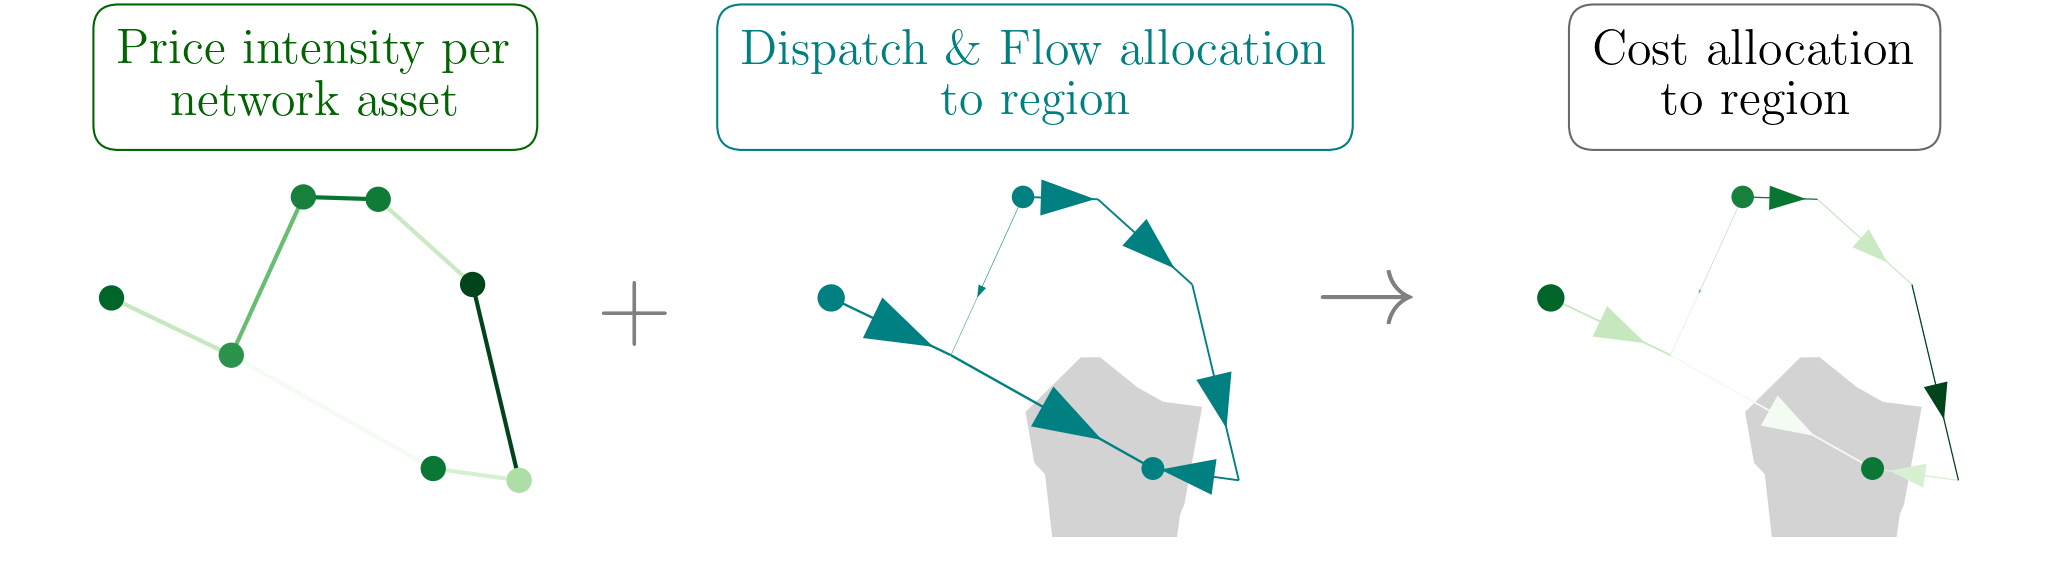
\includegraphics[width=\linewidth]{graphical_abstract.png}
          }%
        }
        
    \end{abstract}
 
\end{@twocolumnfalse}
]


\subsection*{Highlights}
\begin{itemize}
    \item In short and long-term equilibria, locational marginal prices determine the revenues of network assets. 
    \item Flow tracing is used to allocate the revenue for each asset separately to consumers. 
    \item The new method decomposes the electricity price at each node in a fair and transparent manner.
    \item Four use-cases are proposed and demonstrated on behalf of a future model of the German power system. 
\end{itemize}


\subsubsection*{Nomenclature}

\begin{table}[h!]
    \centering
    \begin{tabular}{ll}
        $\lmp$ & Locational Market Price at bus $n$ and  \\ & time step $t$ in \euro/MW \vpad \\
        $\demand$ & Electric demand at bus $n$ \\ & time step $t$ in MW  \vpad \\
        $\nodalgeneration$ & Electric generation of all generators at bus $n$, \\ & time step $t$  in MW \vpad \\
        $\generation$ & Electric generation of generator $s$, \\ & time step $t$  in MW \vpad \\
        $\flow$ & Active power flow on line $\ell$,\\ &time step $t$ in MW   \vpad \\
    \end{tabular}
\end{table}

\section{Introduction}

Today's power systems are subject to a deep and ongoing transformation. The shift from controllable to variable, weather-driven power generation as well as the constant improvement and innovation of technology require rigorous system planning and international cooperation \cite{pfenninger_energy_2014,schlachtberger_benefits_2017}. The core of the challenge manifests in the total costs of the system. Firstly, these should be as low as possible while meeting ecological and techno-economic standards. Secondly, they must be distributed in a fair and transparent manner among all agents in the power system. It is central to identify the drivers of costs and address them appropriately.  
In this respect, power system models are a valuable and widely used tool \cite{pfenninger_energy_2014,bazmi_sustainable_2011,pereira_generation_2017,brown_sectoral_2019}. Many studies for countries and regions throughout the world exist that lay out how renewable energy penetration can be expanded at minimum costs. Yet they largely remain silent how and on which grounds these costs are allocated among consumers. 

This paper fills this gap. We present a new method, named Price Tracing, which interlinks the electricity prices between different nodes for single time steps. The method builds upon Bialek’s \ac{AP} \cite{bialek_tracing_1996}, also known as Flow Tracing, and weights the power flow allocations with the \ac{LMP}. This builds the basis for a transparent disentanglement of cost contributions to the consumer electricity prices, \textit{i.e.} it does not only answer the question of who delivers power to whom but also how much the consumers have to pay to specific generators or transmission lines. 

The literature discussed and applied the concept of flow-based cost allocation in a range of papers \cite{galiana_transmission_2003,shahidehpour_market_2002,meng_investigation_2007,schafer_allocation_2017,nikoukar_transmission_2012,arabali_pricing_2012,wu_locational_2005}. Shahidehpour et al. provide a profound insight into allocating congestion cost and transmission investments to market participants using different allocation techniques \cite{shahidehpour_market_2002}. Specifically, they set out that Generation Shift Factors, i.e. the marginal contribution of generators to a flow on line, allow to represent the \ac{LMP} as a superposition of the \ac{LMP} at the reference bus, the price for congestion and a price for losses. The approach in \cite{meng_investigation_2007} expands this relation for contributions based on the \ac{AP} scheme, which allows for an accurate, however inexact, estimation of the optimal \ac{LMP}. A similar approach is used in \cite{schafer_allocation_2017} that allocates electricity prices of a non-optimal power dispatch based on \ac{AP}.


In this paper, we bring together the advantages of the studies discussed above. Our approach assures localized cost allocations while fully aligning payments to the nodal pricing scheme based on the \ac{LMP}. It serves to facilitate transparency and cost-benefit analysis in network plannings such as the Ten Year Network Development Plan \cite{entso-e_completing_2020} or the German Netzentwicklungsplan \cite{bundesnetzagentur_netzentwicklungsplan_2020}. Further, it provides a point of departure for usage-based transmission cost allocation.

At first, we formulate the Price Tracing method (\cref{sec:price_tracing}) with underlying assumptions and a numerical example (\cref{sec:numerical_example}). In \cref{sec:application_case} we showcase possible application cases on the basis of an optimized German power system with a high share of renewable power generation. \Cref{sec:limitations} depicts methodogical limitations and \cref{sec:conclusions} draws final conclusions. 


\section{Price Tracing}
\label{sec:price_tracing}

Assume an electricity network with N nodes, L lines and T time steps. Using the linearized power flow approximation, the power flow $\flow$ on a passive line $\ell$ at time $t$ relates to the generation $\nodalgeneration$ and demand $\demand$ at node $n$ and time $t$ according to 
\begin{align}
    \flow = \sum_n \ptdf \left(\nodalgeneration - \demand \right) \Forall{t}
\end{align}
where $\ptdf$ are the \ac{PTDF}. These translate the nodal injection on the right hand side to the network flow in compliance with the linearized Kirchhoff Circuit Laws. 
% \ac{KCL} and \ac{KVL}.
% \footnote{for transport models or networks with \acl{HVDC} lines, these can be artificially derived from the network flow using the formulation in \cite{hofmann_flow_2020}}

In a nodal pricing scheme, the system cost occasioned by the electrical demand $\demand$ is proportional to the corresponding \ac{LMP} $\lmp$, 
\begin{align}
    \text{Demand Cost}: \lmp\, \demand .
    \label{eq:demand_cost}
\end{align}
On the other hand, system assets gain a revenue from their operation. Therefore, the revenue of the dispatch $\nodalgeneration[m]$ at bus $m$ is given by 
\begin{align}
    \text{Dispatch Revenue}: \lmp[m] \, \nodalgeneration[m] 
    \label{eq:dispatch_revenue}
\end{align}
and the congestion revenue of line $\ell$ at time $t$ by 
\begin{align}
    \text{Congestion Revenue}: \lmp[\ell]\, \flow .
    \label{eq:congestion_revenue}
\end{align}
where in the absence of network cycles the revenue per transported MWh $\lmp[\ell]$ is the price difference $\lmpdiff$ between ending and starting node of line $\ell$. In case of network cycles, the price of the \ac{KVL} $\lmpkvl$ may be added to $\lmp[\ell]$ to adjust congestion revenues to expenditures in a long-term equilibrium, see \cref{sec:problem_formulation,sec:zero_profit_flow} for details. The \ac{LMP} as well as the prices for the \ac{KVL} are given by the dual values, often related to as shadow prices, of the corresponding constraints in the underlying cost-optimization (see \cref{sec:optimality_conditions} for details).   
% Using the Incidence Matrix $\incidence$, which is 1 if $n$ is a starting node of line $\ell$, -1 if $n$ is a ending node of line $\ell$ and zero otherwise, the price differences are given by $\lmpdiff = - \sum_n \incidence \lmp$.

Naturally, the sum of all demand costs at time $t$ equal the sum of all revenues at time $t$, that is 
\begin{align}
    \sum_{n} \lmp\, \demand  = \sum_{m} \lmp[m]\, \nodalgeneration[m] + \sum_{\ell} \lmp[\ell]\, \flow \Forall{t} .
    \label{eq:total-demand-cost}
\end{align}
This equality relates the sum of costs to the sum of revenues, however the relationships between individual contributions on the left hand side and individual contributions on the right hand side remain undefined. The following shows that by allocating flows in the network, it is possible to relate the power consumption at single nodes to the revenues of single generators and transmission lines: 

We start with the fact that dispatch and flow can be considered as a superposition of individual contributions of nodes and assets. The literature provides various methods, called \ac{FA} method, to artificially quantify these. Each method follows a particular set of assumptions that lead to \ac{P2P} allocations $A_{m \rightarrow n}$ which measure the power generated at node $m$ and consumed at node $n$. Flow Tracing, also known as \ac{AP} \cite{bialek_tracing_1996}, is a flow allocation method that traces the power injection at bus $m$ through the network up to its sink $n$ using the principle of proportional sharing. The method is illlustrated in \cref{fig:ap-scheme} and mathematically documented in \cref{sec:net_ap}. 

\begin{figure}
    \centering
    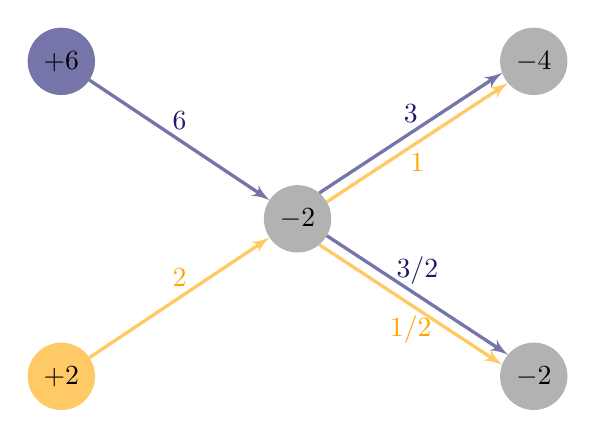
\begin{tikzpicture}

        % vertices
        \node[vertex, draw=Orange!60, fill=Orange!60] (1) at (0,0) {$+2$};
        \node[vertex, draw=MidnightBlue!60, fill=MidnightBlue!60] (2) at (0,4) {$+6$};
        \node[vertex, draw=Gray!60, fill=Gray!60] (3) at (3,2) {$-2$};
        \node[vertex, draw=Gray!60, fill=Gray!60] (4) at (6,0) {$-2$};
        \node[vertex, draw=Gray!60, fill=Gray!60] (5) at (6,4) {$-4$};
        
        %edges
        \draw[edge, draw=Orange!60] (1) -- (3) node[midway, above] {\color{Orange}$2$};
        \draw[edge, draw=MidnightBlue!60] (2) -- (3) node[midway, above] {\color{MidnightBlue}$6$};
        \draw[edge, draw=MidnightBlue!60] (3.330) -- (4.140) node[midway, above] {\color{MidnightBlue}$3/2$};
        \draw[edge, draw=Orange!60] (3.310) -- (4.160) node[midway, below] {\color{Orange}$1/2$};
        \draw[edge, draw=MidnightBlue!60] (3.050) -- (5.200) node[midway, above] {\color{MidnightBlue}$3$};
        \draw[edge, draw=Orange!60] (3.030) -- (5.220) node[midway, below] {\color{Orange}$1$};
    \end{tikzpicture}
    \caption{Schematic illustration of the \ac{AP} method. Figuratively, each power source is given one color. As soon as different power flows mix at a node, the mix of ``colors'' in the outgoing flows are in proportion to the ingoing flows. Therefore, all consumed power can be related to a distinct origin.}
    \label{fig:ap-scheme}
\end{figure}

When flows from different sources meet at the same bus, their proportion determines the mix of all outgoing flows from this bus, including nodal withdrawal. The advantage of the \ac{AP} method is the spatial confinement of \ac{P2P} allocations $A_{m \rightarrow n}$ \cite{hofmann_techno-economic_2020}. Naturally, the sum of all recipients yields the nodal generation at $m$, thus
\begin{align}
    \nodalgeneration[m] = \sum_n \allocatepeer \Forall{m.t} 
    \label{eq:nodalgeneration-breakdown}
\end{align}   
For reasons to follow, we resort only to \ac{P2P} mappings of the \ac{AP} method. Thus, regardless of the \ac{AP} allocation, let $\allocateflow$ denote the flow contribution of demand $\demand$ such that the sum of all flow contributions equals flow on line $\ell$,  
\begin{align}
    \flow = \sum_n \allocateflow \Forall{\ell,t}.
    \label{eq:flow-breakdown}
\end{align}
We substitute \cref{eq:nodalgeneration-breakdown,eq:flow-breakdown} into \cref{eq:total-demand-cost} and impose that the equality holds separately for all summands referring to $n$ which leads us to 
\begin{align}
    \lmp\, \demand &= \sum_m \lmp[m] \allocatepeer + \sum_\ell \lmp[\ell] \allocateflow \Forall{n,t}
    \label{eq:demand-cost-allocation}
\end{align}
This equation maps the cost of nodal demand on the left-hand side to the contributions of dispatch and congestion revenues on the right-hand side. It thus indicates what consumers at $n$ have to pay to generators at $m$ and the transmission line $\ell$. The equation introduces N new equalities for each time step of which the necessary degree of freedom comes from the yet undefined flow contribution $\allocateflow$. In \cref{sec:proof_equivalence} we proof that 
\begin{align}
    \allocateflow = \sum_m \ptdf[m] (\allocatepeer - \delta_{nm} \demand) 
    \label{eq:allocateflow}
\end{align}
solves \cref{eq:demand-cost-allocation} where $\delta_{mn}$ is 1 for $m=n$ and zero otherwise. We see that the flow contribution $\allocateflow$ follows from the \ac{P2P}-assignment $\allocatepeer$. Thus, the contributions of dispatch and congestion revenue to the demand cost in \cref{eq:demand-cost-allocation} can be expressed as a function of the \ac{LMP} $\lmp$ and the \ac{P2P} allocation $\allocatepeer$. Note that this holds true because the allocations on lines given in \cref{eq:allocateflow} obey the (linearized) \ac{KVL}\footnote{for transport models or networks with \acl{HVDC} lines, the PTDF can be artificially derived from the network flow using the formulation in \cite{hofmann_flow_2020}}. In contrast, the flow allocations given by the \ac{AP} method do not respect the \ac{KVL} as already stated by \cite{galiana_transmission_2003}, thus do not hold \cref{eq:demand-cost-allocation}\footnote{This also explains the inexact cost estimation in \cite{meng_investigation_2007} which are purely based on the flow contributions of the \ac{AP} method.}. 

Following the formulation in \cite{schafer_tracing_2020}, a \ac{P2P}-assignment $\allocatepeer$ breaks down into contributions $\allocategeneration$ from generator $s$ to demand at $n$ which are set in proportion to the contribution of generator $s$ to $\nodalgeneration[m]$. The new allocation then fulfills
\begin{align}
    \generation = \sum_n \allocategeneration
    \label{eq:generation-breakdown}
\end{align}  
with $\generation$ being the output of generator $s$ at time $t$. \\


The \textit{Price Tracing} method for a network with a linearized power flow and a nodal pricing scheme builds on the above equations and defines  
\begin{subequations}
    \begin{align}
    \allocategeneratorcost = \lmp[s] \allocategeneration
\end{align}
as the payment from consumers at $n$ to generator $s$ as well as  
\begin{align}
    \allocatelinecost = \lmp[\ell] \allocateflow
\end{align}
\end{subequations}
as the payment to transmission line $\ell$. For consistency, let $\payment = \lmp \demand$ denote the nodal payment of all consumers at node $n$ which according to \cref{eq:demand-cost-allocation} is $\payment = \sum_s \allocategeneratorcost + \sum_\ell \allocatelinecost$. 

Note that storage units such as batteries may be easily introduced into the Price Tracing method: When they discharge power, they are treated like generators and when they charge power, they are treated like consumers. For the latter, the allocations $\allocategeneration$ and $\allocateflow$ must be divided into allocations to consumers and charging storage units at $n$.    

% Price Tracing enables to track the flow of money in a network with optimal or sub-optimal prices. Note that as long as the allocation $\allocatepeer$ fulfills \cref{eq:flow-breakdown,eq:generation-breakdown}, it may be modified. So, there is a degree of freedom to pre-allocate direct \ac{P2P} tradings $\allocatepeer^\text{Trade}$ and to allocate the remaining generation and demand with the \ac{AP} method, thus 
% \begin{align}
%     \allocatepeer = \allocatepeer^\text{Trade} + \allocatepeer^\text{AP} .
% \end{align}
% This optional modification leads to a Price Tracing which includes exchanges between \ac{P2P} traders as well as ordinary market participants. 


\subsection{Numerical Example}
\label{sec:numerical_example}

In the following we illustrate the Price Tracing method in a numerical example and start with a three node network with two lines. We optimize the dispatch for one time step and perform the cost allocation. We then add a third line to the system and repeat the cost allocation to show the effect of the network cycle.      


\subsubsection*{Network without Cycles}
\Cref{fig:example-network} shows the optimized three-node network with corresponding numerical values.
\begin{figure}[h!]
    \includegraphics[width=\linewidth]{example-without-cycles/network.png}
    \caption{Example network with nodal pricing scheme. Dispatch revenue as well as demand cost per MWh are given by the \ac{LMP} $\lambda$. Congestion revenue per MWh is given by the price difference $\lambda^\text{diff}$ of the connecting nodes.}
    \label{fig:example-network-wo}
\end{figure}
Both, bus 1 and 2 have a fixed demand of 30~MW and 50~MW, respectively. Bus 1 has a generator with a marginal price at 6 \euro/MWh. Bus 3 has a cheaper generator with marginal price at 4 \euro/MWh. The maximal capacity of both generators is 50 MW. The transmission line from 1 to 2 has a capacity of 60\,MW and line from 3 to 1 a capacity of 30 MW. Since the latter limits the use of the cheaper generator, there is a price difference between bus 1 and 3 of 2 \euro/MWh. Due to the absence of network cycles, this price difference defines the congestion revenue of line 3--1. Line 1--2 is not bound, hence there is no congestion revenue and bus 2 and 1 have the same electricity price of 6 \euro/MWh.  

According to the \ac{AP} method, the demand at bus~1 is supplied by the local generator. In contrast, bus~2 imports power from bus~1 and bus~3. Using the Price Tracing method, we calculate the cost allocations $\mathcal{C}_{n\rightarrow s}$ and $\mathcal{C}_{n\rightarrow \ell}$, which we show in \cref{fig:example-network-payoff-wo}. Consumers at bus~1 only have to compensate the local generator with 180 \euro. Consumers at bus~2 pay for congestion revenues of line 1--3, all electricity generation at bus~3 and the remaining dispatch revenues of the generator at bus~1.    

\begin{figure}[h]
    \includegraphics[width=\linewidth]{example-without-cycles/payoff.png}
    \caption{Allocation matrices $\mathcal{C}_{n\rightarrow s}$ (left) and $\mathcal{C}_{n\rightarrow \ell}$ (right) for the dispatch and congestion revenue for the network in \cref{fig:example-network-wo}.}
    \label{fig:example-network-payoff-wo}
\end{figure}

The consistency of the cost allocation can be easily double-checked. The sum of a column  yields the payment to a generator or a line. This exactly matches the dispatch and congestion revenue defined in \cref{eq:dispatch_revenue,eq:congestion_revenue}. In turn the sum of a row gives the total amount that consumers at a bus have to pay. These exactly match the demand cost $\lambda_n \, d_n$. For example the sum of payments of consumers at bus~2 is 300~\euro\, which is the price of 6~\euro/MWh times the consumption of 50~MWh. \\



\subsubsection*{Network with Cycle}

Now, we add a line from bus~3 to bus~2 with a capacity of 30~MW. This introduces a \ac{KVL} constraints for the three lines, requiring that the sum of flows following the cycle is zero\footnote{For simplicity we assume a uniform impedance in the example.}. As shown in \cref{fig:example-network} the new line capacity is bounded at 30~MW. The new cost optimum results in a higher price at bus~2 of 8~\euro/MWh despite that the cheaper generator~2 produces 10~MW more than before. This result may be counterintuitive, but it becomes clear when considering that the new line's low capacity limit of 30~MW, combined with the \ac{KVL}, restricts flow on lines 1--3 and line 1--2.   

\begin{figure}[h!]
    % \begin{subfigure}[c]{0.5\linewidth}
        \includegraphics[width=\linewidth]{example-with-cycles/network.png}
        \caption{Example network with nodal pricing scheme and a network cycle. Now, due to the \ac{KVL} a new constraint adds to the optimzation problem. Optionally, the congestion revenue per MWh may include shadow prices of the \ac{KVL} constraint $\lmpkvl$, thus $\lmp[\ell] = \lmpdiff + \lmpkvl$.}
        \label{fig:example-network}            
    % \end{subfigure}
\end{figure}

\begin{figure}[h!]
    \begin{subfigure}[c]{\linewidth}
        \includegraphics[width=\linewidth]{example-with-cycles/payoff.png}
        \subcaption{Without \ac{KVL} shadow prices}
        \label{fig:example-network-payoff}
    \end{subfigure}
    \begin{subfigure}[c]{\linewidth}
        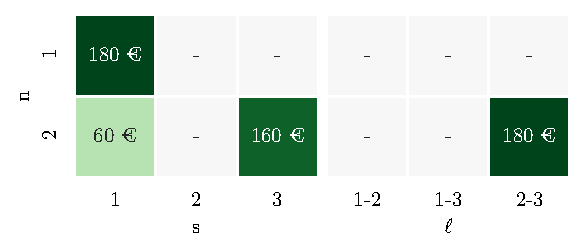
\includegraphics[width=\linewidth]{example-with-cycles/payoff-kvl.png}
        \subcaption{With \ac{KVL} shadow prices}
        \label{fig:example-network-payoff-kvl}
    \end{subfigure}
    \caption{Cost allocations $\allocategeneratorcost$ and $\allocatelinecost$ for the dispatch and congestion revenue for the network in \cref{fig:example-network}.}
    \label{fig:example-network-payoff-all}
\end{figure}

The prices $\lambda_\ell^\text{KVL}$ of line $\ell$ are returned as the shadow price of the \ac{KVL} constraints in the cost-optimization, see \cref{sec:problem_formulation} for details. The Price Tracing method optionally allows to consider these in the congestion revenue without loosing its consistency with the demand costs. 



\Cref{fig:example-network-payoff} shows the cost allocation without considering the \ac{KVL} shadow prices. Here, the congestion revenue is proportional to the price difference of the connected buses and congestion revenue of the new line 2--3 is the highest at 120~\euro/MWh. In contrast \cref{fig:example-network-payoff-kvl} shows the cost allocation under consideration of the \ac{KVL} shadow prices. Here, the congestion revenues are shifted towards 1--2 and 1--3. Note that this shift accounts for the fact that it is in fact the new line 2--3 that limits the flow on line 1--2 and 1--3.    

Again both cost allocation schemes are consistent with the total demand cost, dispatch and congestion revenues. In the following, we consider the \ac{KVL} shadow prices in the Price Tracing method since then, the total congestion revenue of a line equals the sum of all associated line costs in a short and long-term equilibrium.  

\begin{figure*}[h!]
    \centering
    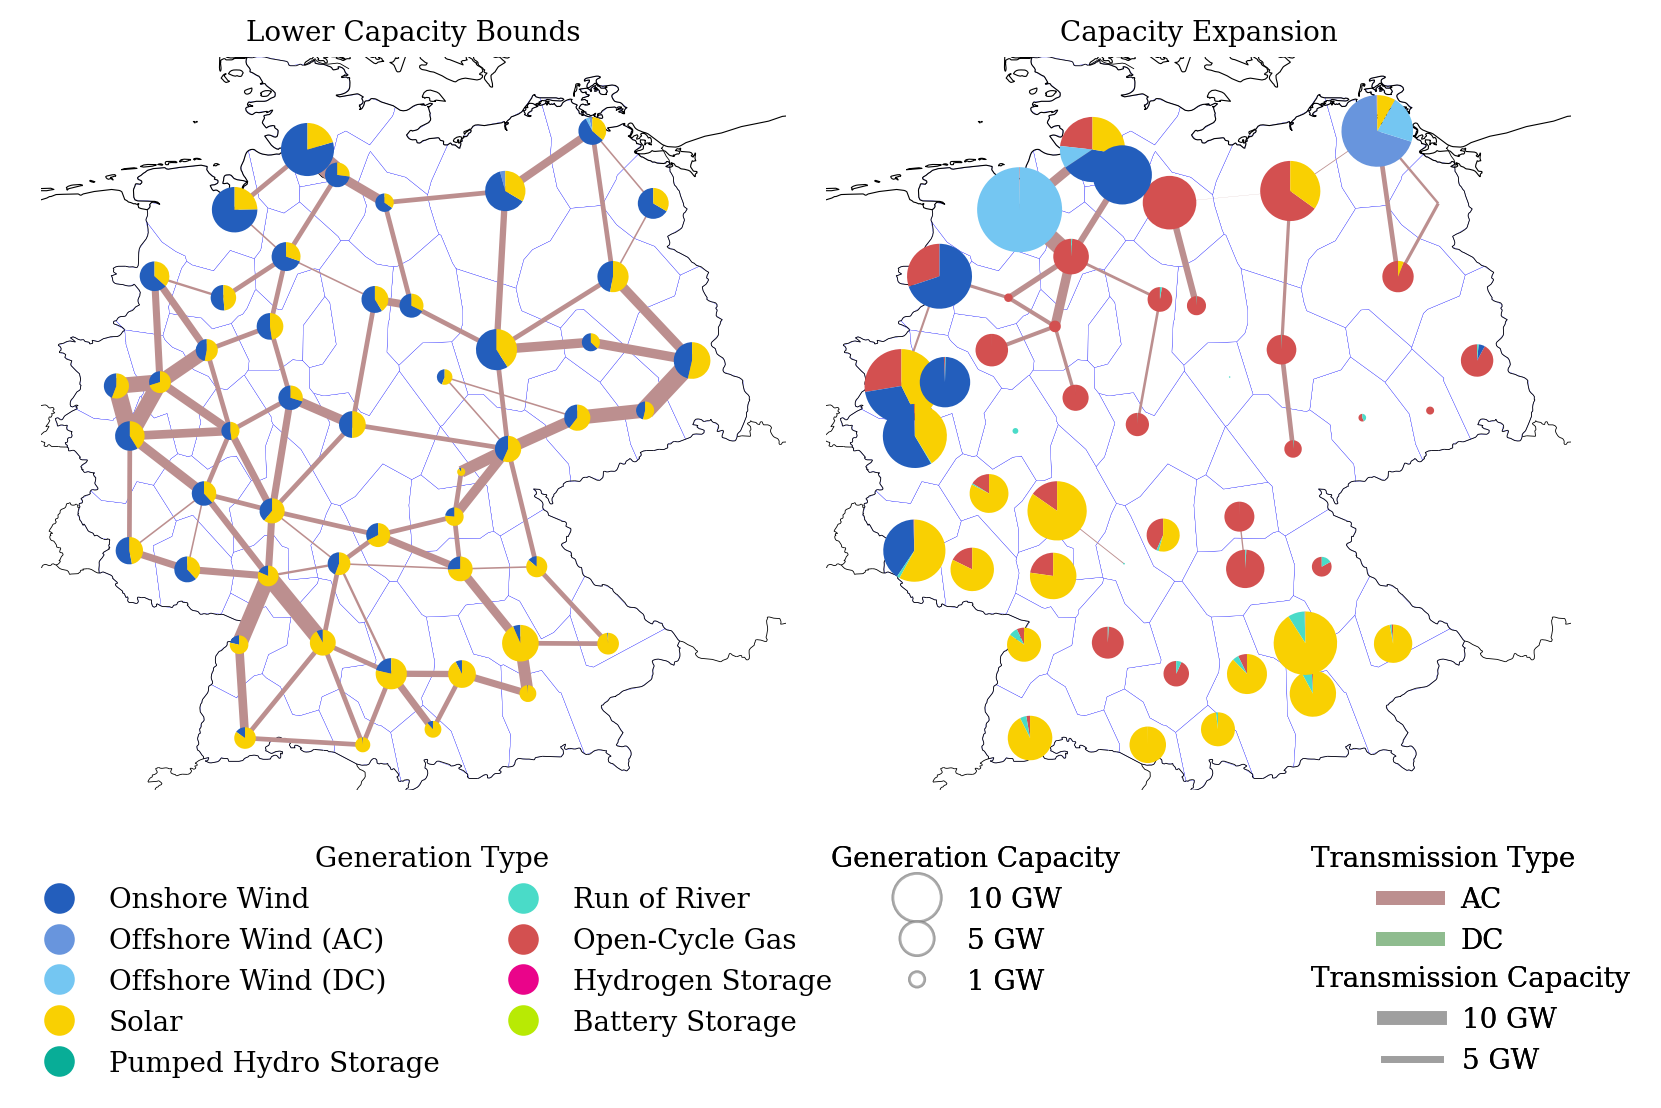
\includegraphics[width=\linewidth]{de50/network}
    \caption{Model of the German power system. The left hand side shows minimum requirements for renewable and transmission capacities. The right hand side shows the cost-optimal capacities of all generators as well as transmission expansions. The effective CO$_2$ price is set to 120 \euro\, per tonne CO$_2$ emission.}
    \label{fig:network}
\end{figure*}
 

\section{Application Cases}
\label{sec:application_case}

Using a cost-optimized model of the German power system with 50 representative nodes and a one year time span with hourly resolution, we demonstrate four use cases of the Price Tracing method. 

The investment model builds up on the PyPSA-EUR workflow \cite{horsch_jonas_pypsa-eur_2020} whose technical details and assumptions are presented in \cite{horsch_pypsa-eur_2018}. Transmission line capacities can be expanded but require a minimum of today's capacities, originally retrieved from the ENTSO-E Transmission System Map \cite{entso-e_entso-e_nodate}. Further, we require a minimum deployment of renewable capacity derived from matching all entries of the OPSD renewable power plant list \cite{schlechtRenewablePowerPlants2020} to its closest bus. Wind and solar capacity expansion are limited by land-use restrictions considering agriculture, urban, forested and protected areas based on the CORINE and NATURA2000 database \cite{eea_corine_2012,eea_natura_2016}. \ac{PHS} and \ac{ROR} power plants are fixed to today's capacities and may not be expanded. Additionally, unlimited expansion of batteries and H$_{2}$-storages and \ac{OCGT} are allowed at each node. 
% 
% 
\begin{figure}
    \centering
    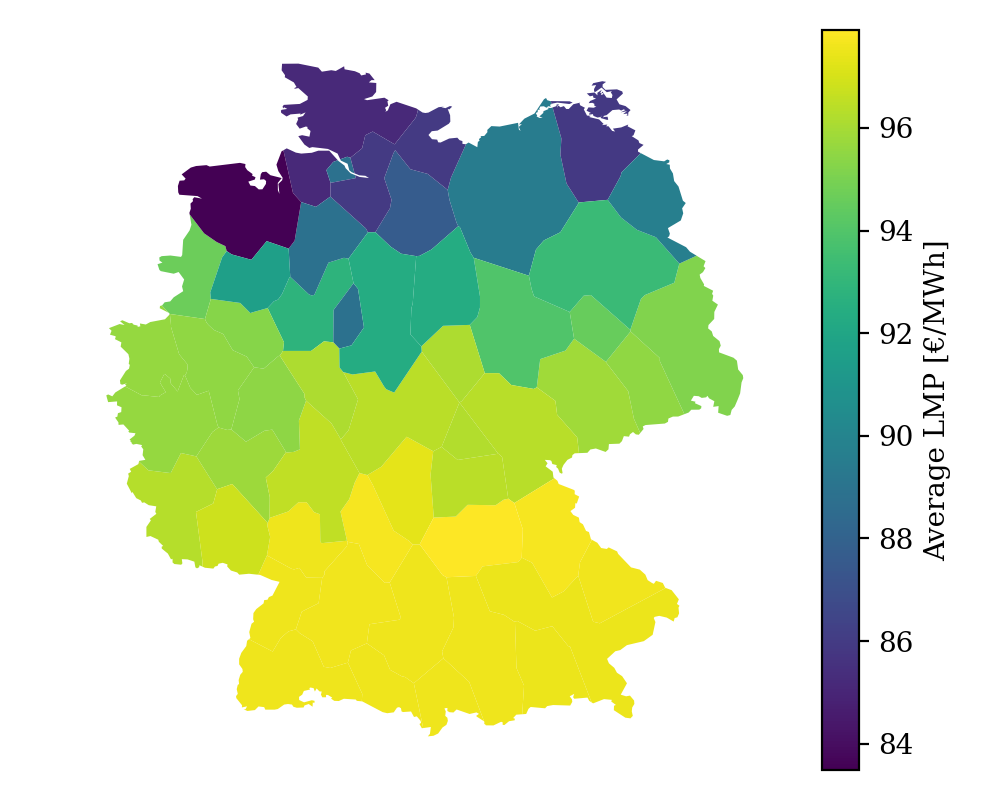
\includegraphics[width=\linewidth]{de50/average_price}
    \caption{Load-weighted average electricity price $\averagelmp$ per region in the optimized German power system. Regions in the middle and south of Germany have high prices whereas electricity in the North with a strong wind, transmission and \ac{OCGT} infrastructure is cheaper.}
    \label{fig:average_price}
\end{figure}
We impose a carbon price of 120 \euro\, per tonne-CO$_{2}$ which, for OCGT, adds an effective price of 55 \euro/\megawatthour (assuming a gross emission of 180~kg/MWh and an efficiency of 39\%). All cost assumptions on operational costs $o_i$ and annualized capital cost $c_i$ are summarized in \cref{tab:cost_assumptions}. 

The network is shown in  \cref{fig:network}. The left hand side shows all minimum capacity requirements, the right hand side the cost-optimal capacities. Solar capacities are expanded in the south, onshore and offshore wind in the upper north and far west. \ac{OCGT} are built in the middle and north of the country. Transmission lines are amplified along the north-south axis, including a major \ac{DC} link, associated with the German S\"ud-Link, running from the coastal region to the southwest. 
The total annualized cost of the power system roughly sums up to 46 billion \euro.
% 

\Cref{fig:average_price} displays the load-weighted average electricity price $\averagelmp$ per region, defined by 
\begin{align}
    \averagelmp = \dfrac{\sum_{t} \lmp \demand}{\sum_t \demand} = \dfrac{\sum_{t} \payment }{\sum_t \demand}    
\end{align}
It reveals a relatively strong gradient from south (at roughly 98 \euro/MWh) to north (84 \euro/MWh). Regions with little minimum capacity requirements and little capacity expansion, especially with respect to renewable generation, tend to have higher prices. 
% The node with the lowest \ac{LMP} in the upper northwest, stands out through high offshore capacity requirements.
 \\
 
\subsection{Usage-based Network Tariff}

The first possible use-case of the Price Tracing method we discuss here, is a usage-based network tariff. Among other countries, electricity consumers in Germany pay a uniform network tariff, the ``Netzentgelte''. These are based on an relatively opaque calculation and valuation of all network cost for each Transmission System Operator, in addition to a individually derived profit margin. 

The Price Tracing method allocates all congestion revenues to consumers in the network, given by $\allocatelinecost$. This cost allocation can be used to define a usage-based network tariffs $\averagelmp^\text{grid}$ for each bus-region $n$ in the network:     
\begin{align}
    \averagelmp^\text{grid} = \dfrac{\sum_{t,\ell} \allocatelinecost}{\sum_t \demand}.
\end{align}
This is the average price that consumers at $n$ pay for the transmission of electricity. These include compensations for all capital investments taken by the network operators. Consumers with a high degree of nodal autarky, \ie with a little net electricity import, pay a lower network tariff and vice versa. This gives an incentive to regions with a sub-optimal deployment of renewable technologies to invest in local infrastructure. Note since the cost-optimum represents a long-term equilibrium, the total revenue per network asset equals the total \ac{OPEX} and \ac{CAPEX}. Therefore, the network tariffs $\averagelmp^\text{grid}$ do not result in any profits. 

A further advantage of this network tariff allocation lays in the possibility to differentiate between different network operators. The quantity 
\begin{align}
    \averagelmp[n\rightarrow \ell]^\text{grid} = \dfrac{\sum_{t} \allocatelinecost}{\sum_t \demand}
\end{align}
decomposes the network tariff to single lines, naturally fulfilling  $\averagelmp^\text{grid} = \sum_\ell \averagelmp[n\rightarrow \ell]^\text{grid}$. This facilitates to trace back which congested lines are the strongest drivers to the local network tariff.   

Figure ... shows the network tariffs for all regions of the showcase model. 


\subsection{CO$_2$-Cost Allocation}
\label{sec:co2-cost-allocation}

\begin{figure}[h!]
    % 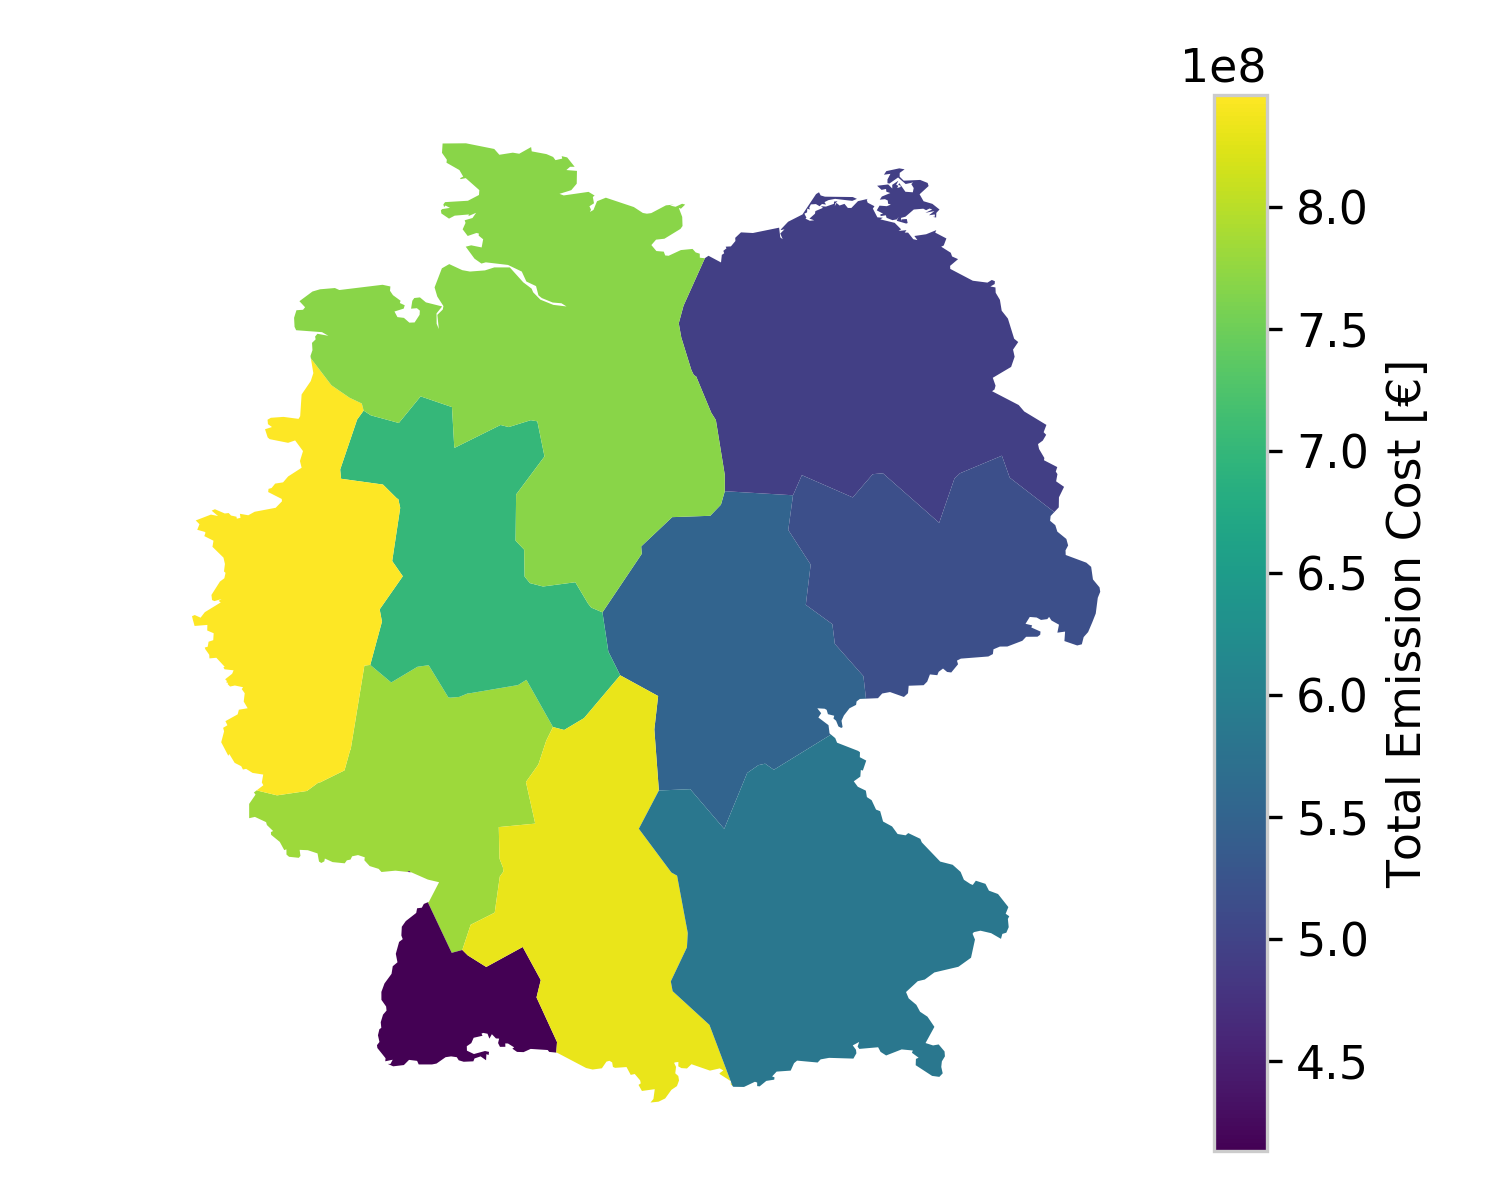
\includegraphics[width=\linewidth]{de50/maps_price_ptpf_net/co2_cost_total.png}
    \caption{Average CO$_2$ cost per consumed MWh. The effective prices are indicated by the color of the region, the circles are drawn in proportion to the revenue per regional generators.}
    \label{fig:opex_price}
\end{figure}

The mapping $\allocategeneratorcost$ allocates all dispatch revenues from generators to consumers. Naturally, the revenues of conventional generators include costs accounting for CO$_2$ emissions. Using the mechanism of the Price Tracing method, these CO$_2$ costs may be mapped to the consumers by weighting the dispatch allocation $\allocategeneration$ with the effective CO$_2$ price $\emissionprice$ per produced MWh at generator $s$. Applying an emission cost allocation in the form of     
\begin{align}
    \allocateemissioncost = \emissionprice \allocategeneration
\end{align}       
into a power system, incentivizes consumers to reduce their emission intensive power consumption and leads to a transparent polluter pay principle. The average emission cost per consumed MWh is given by 
\begin{align}
    \averagelmp^{\text{CO}_2} = \dfrac{\sum_{t,\ell} \allocateemissioncost}{\sum_t \demand}.
\end{align} 
\Cref{fig:opex_price} depicts the price for the showcase model. It is very much aligned with the deployment of \ac{OCGT} generators whose revenue from emissions is indicated by the size of the circles.   
Note, that such a CO$_2$ price tracing could also be applied to networks without a nodal pricing scheme.  



\subsection{A Transparent Nodal Pricing Scheme}


\begin{figure*}[h!]
    \centering
    \begin{subfigure}[c]{.6\linewidth}
    % \includegraphics[width=\linewidth]{de50bf/ptpf_net_to_lowest-lmp}
    \end{subfigure}
    \hspace{-.2151\linewidth}
    \begin{subfigure}[c]{.6\linewidth}
    % \includegraphics[width=\linewidth]{de50bf/ptpf_net_to_highest-lmp}
    \end{subfigure}
    \caption{Comparison of payments of the region with the \textbf{lowest LMP (left)} and the region with the \textbf{highest LMP (right)}. The region is colored in dark blue. The circles indicate to which bus and technology the payments are assigned. The thickness of the lines is proportional to dedicated payments.}
    \label{fig:direct-allocation}
\end{figure*}

A third presented application case of the Price Tracing method is to make the nodal demand cost in a network more transparent. To demonstrate this, \cref{fig:direct-allocation} shows the total \ac{P2P} cost assignments $\sum_t \allocategeneratorcost$ and $\sum_t  \allocatelinecost$ of the region with the lowest average \ac{LMP} (left side) and the one with the highest \ac{LMP} (right side). 

Due to its small net imports, the low-price region in the north-west hardly pays for congestion revenues. It profits from local offshore wind farms and only a small share of the payments is allocated to remote \acp{OCGT}. In contrast, the high-priced region is highly dependent on local \ac{OCGT} and the transmission system, which causes high allocated dispatch and congestion revenues. Interestingly, its payments to  onshore and offshore wind infrastructure are low despite a third of its supply comes from wind power. This leads to the conclusion, that wind power supply at this region is not restricted by exhausted wind power resources but by bottlenecks in the transmission system.  




% Finally, \cref{fig:locality} draws the cumulative share of P2P cost assignments of a function of the distance between producer and consumer. The data is shown for all technologies separately. The later the curve reaches 100\% the deeper the price of a technologies penetrates into the network. Offshore wind has the strongest price influence to remote buses. Only 10-30\% of its expenses are compensated by local consumers and the rest is assigned to remote buses, especially those with high demand (compare \cref{fig:average_demand}). The contrast between Hydrogen Storage and Battery sticks out. Whereas Battery costs are hardly assigned to other buses, almost 50\% of the Hydrogen Storage costs are payed by remote buses. It underlines the fundamental functionality of the two technologies. Hydrogen storage are located at buses with high wind generation and balance out their long-term excess and deficit energy. The dispatched power follows a similar way through the network as the wind power. The battery on the other hand pairs with local solar production and its locally constraint dispatch and flow.     

% \begin{figure}
%     \centering
%     \includegraphics[width=\linewidth]{de50bf/locality_all_ptpf_net}
%     \caption{Average distance between payer and receiver for different technologies and shares of the total production.}
%     \label{fig:locality}
% \end{figure}




\subsection{Revenue Decomposition}

Finally, we demonstrate a optimization related application case of the Price Tracing method which focuses on decomposing the congestion and dispatch revenue. In a long-term equilibrium without any exogenous constraints, an network asset recovers all its \ac{OPEX} and \ac{CAPEX} from the revenue. This relation is known as the zero-profit rule and is an outcome of the \ac{KKT} conditions of the underlying cost-minimization problem derived in detail in \cref{sec:zero_profit_generation,sec:zero_profit_flow,sec:zero_profit_storage_units}. However, if the cost-optimum is constrained exogenously, for example by minimum share of renewable capacity, the zero-profit rule is shifted and more cost contributions have to be considered \cite{brown_decreasing_2020} as soon as the new constraint becomes binding. 

\begin{table}[h!]
    \caption{Exemplary contributions to the revenue of network assets highlighted in this work. Depending on the formulation of the optimization problem, the list changes and may possibly include other terms.}
    \begin{center}
        \begin{tabular}{c|c p{0.3\textwidth}}
            \toprule
            \text{Contribution} & Symbol \\
            \midrule
            \text{OPEX} & $\opex$ \\
            % \midrule
            \text{CAPEX} & $\capex$ \\
            % \midrule
            \text{Emission Tax} & $\emissioncost$ \\
            % \midrule 
            \text{Scarcity Rent} & $\scarcitycost$ \\
            \text{Subsidies} & $\subsidycost$ \\
            \vdots & \vdots \\
            \bottomrule
        \end{tabular}                
    \end{center}
    \label{tab:contributions}
\end{table}

\noindent
\Cref{tab:contributions} shows a possible set of contributions to the demand costs which relate to the congestion and dispatch revenue in a investment problem. On top of \ac{OPEX} and \ac{CAPEX} we display the emission cost which we already discussed in \cref{sec:co2-cost-allocation}. In the presence of capacity expansion limits, additional Scarcity Rent $\scarcitycost$ has to be considered in the revenue, in case the corresponding constraints are binding. This rent translates to a compensation for higher competed investments, but can also be ignored in case an asset is fixed to its existent, amortized capacity, see \cref{sec:upper_capacity_limits}. Likewise, assets may be constrained to lower capacity requirements which reflect \ie  existing infrastructure known as Brownfield constraints, see \cref{sec:lower_capacity_limits}. If bounded, the lower limit reduces the revenue of the corresponding asset and leaves a Subsidy Cost $\subsidycost$ which have to compensated by external institutions (government, community) or are simply ignored in case the asset is already amortized. 

Except for the subsidies, all contributions can be expressed in terms of the operation of an asset, thus the generation $\generation$ and the flow $\flow$. Thus, we can decompose the allocated dispatch revenue according to 
\begin{align}
    \allocategeneratorcost = \allocateopex + \allocatecapex + \allocateemissioncost + \allocatescarcitycost - \subsidycost_s .
\end{align} 
APPENDIX shows the individual cost allocations for the showcase model. Note that transmission lines are assumed to have neither \ac{OPEX} nor emission tax, \ie
\begin{align}
    \allocatelinecost = \capex_{n \ra \ell, t} + \scarcitycost_{n \ra \ell, t} - \subsidycost_\ell
\end{align}
The decomposition of the revenue allocation shows how buses remote from wind farms pay higher prices due to increased reliance in transmission and backup capacity. On the other hand, buses with high renewable installation spend most payments to local assets. 



\section{Limitations}
\label{sec:limitations}

The presented cost allocation is based on the linear power flow approximation. Yet, the method is equally applicable to a system with an Optimal Power Flow (OPF), \ie full AC power flows. However, in this case the allocations $\allocategeneration$ and $\allocateflow$ should be computed with the Z-Bus flow allocation presented in \cite{conejo_z-bus_2007} which by design respects both Kirchhoff Circuit Laws. Allocating on the basis of the full power flow introduces an additional cost term accounting for the transmission loss which is compensated by the consumers and mirrors in the \ac{LMP}. 

The used optimization does not take security constrains of the transmission system into account. These may be incorporated following the approach in \cite{nikoukar_transmission_2012}. 

The method can be equally applied to short and long-term planning network models. However, the paper does not take the detailed structure of today's power markets into account. These vary form country to country and often reveal interlocked mechanisms (energy only markets, reserve markets, resdispatch etc.). The aim of the presented work is to reconsider some of the mechanisms and  to reevaluate their market efficiencies.    


\section{Conclusion}
\label{sec:conclusions}

A new method, called Price Tracing, was presented. It decomposes the Locational Marginal Prices in a nodal pricing scheme and the corresponding payments of consumers into dispatch and congestion revenues of individual generators and transmission lines, respectively. It is based on the Average Participation method which calculates assignments between generators and consumers using the principal of proportional sharing. These assignments are weighted with the market price to determine the allocation of the dispatch revenues to consumers. By means of a numerical example, we present the method and show two options of how to treat network cycles in the cost allocation.     

Four application cases of the Price Tracing method were presented, using an optimized model of the German power system with a price of 120~\euro\, per tonne CO$_2$ equivalent. Firstly, it is shown how network tariffs can be adjusted to a transparent, usage-based tariff that give incentives to invest in the local infrastructure. Secondly, the Price Tracing enables to track cost associated with CO$_2$ emissions through the network. This results may be used to reduced CO$_2$ intensive demands in a network. The third presented application case uses Price Tracing to derive cost contributions for individual consumers in order to make nodal payments transparent and explain price differences. This relates to the fourth case where individual dispatch and congestion revenues are decomposed into contributions of operational expenditure, capital expenditure, scarcity rents, subsidies. We show that the allocation can be performed for an individual cost contribution in order to give insights into power system models or to derive political advices.    

\subsubsection*{Reproducibility and Expansion}

All figures and data points can be reproduced by using the \textit{python} workflow in \cite{hofmann_pypsa-costallocation_2020}. The automated workflow allows for higher spatial resolution of the network (scalable up to a the full ENTSO-E Transmission System Map) and optionally taking the total European power system into account.  

\subsection*{Funding}
This research was funded by the by the German Federal Ministry for Economics Affairs and Energy (BMWi) in
the frame of the NetAllok project (grant number 03ET4046A) \cite{bundesministerium_fur_wirtschaft_und_energie_verbundvorhaben_nodate}. 

\subsubsection*{Acknowledgement}

In particular, I thank Tom Brown for very fruitful discussions. I am very grateful to Alexander Zerrahn for reviewing and helping out with important parts. Further, I want to thank Alexander Kies and Markus Schlott who steadily helped with creative thoughts.



% ----------------------- APPENDIX -------------------------------------

\clearpage
\appendix
\subsection*{Acronyms}
\begin{acronym}[UMLX]
    \acro{AC}{Alternating Current}
    \acro{AP}{Average Participation}
    \acro{CAPEX}{Capital Expenditures}
    \acro{CO2}[CO$_2$]{Carbon Dioxide}
    \acro{DC}{Direct Current}
    \acro{FA}{Flow Allocation}
    \acro{HVAC}{High-Voltage Alternating Current}
    \acro{HVDC}{High-Voltage Direct Current}
    \acro{Hydro}{Hydro-Electric Dams}
    \acro{Hydrogen}[H$_2$-storage]{Hydrogen Storage}
    \acro{KCL}{Kirchhoff's Current Law}
    \acro{KKT}{Karush–Kuhn–Tucker}
    \acro{KVL}{Kirchhoff's Voltage Law}
    \acro{LCOE}{Levelized Cost of Electricity}
    \acro{LMP}{Locational Marginal Price}
    \acro{LOPF}{Linear Optimal Power Flow}
    \acro{OCGT}{Open-Cycle Gas Turbine}
    \acro{OPEX}{Operational Expenditures}
    \acro{P2P}{Peer-to-Peer}
    \acro{PHS}{Pumped-Hydro-Storage}
    \acro{PTDF}{Power Transfer Distribution Factors}
    \acro{PV}{Photovoltaic}
    \acro{PyPSA-EUR}{PyPSA-Europe}
    \acro{PyPSA-Eur}{\acs*{PyPSA} Europe}
    \acro{PyPSA}{Python for Power System Analysis}
    \acro{ROR}{Run-of-River}
    \acro{SOAF}[SO\&AF]{\acs*{ENTSO-E} Scenario Outlook and Adequacy Forecast}
    \acro{TSO}{Transmission System Operator}
    \acrodefplural{TSO}{Transmission System Operators}
\end{acronym}




\renewcommand\theequation{\thesection.\arabic{equation}}
\setcounter{equation}{0}

\renewcommand\thefigure{\thesection.\arabic{figure}}    
\setcounter{figure}{0}    

\section{Network Optimization}

\subsection{Optimiality Conditions}
\label{sec:optimality_conditions}

Consider the following linear minimization problem

\begin{align}
    \min_{x_n} \sum_n c_n \, x_n
\end{align}
subject to inequality constraints
\begin{align}
    g_i(x_n) \le 0 \resultsin{\mu_i}
\end{align}
and equality constraints
\begin{align}
    h_j(x_n) = 0 \resultsin{\lambda_j}
\end{align}
where $\mu_i$ and $\lambda_j$ are the corresponding dual variables, also known as \ac{KKT} variables. 
The Lagrangian is given by 
\begin{align}
    \lagrangian = \sum_n c_n x_n + \sum_i \mu_i g_i(x_n) + \sum_j \lambda_j h_j(x_n).
\end{align}

At the optimimum $x^*_n$ the following \ac{KKT} conditions are satisfied. 
\begin{enumerate}
    \item Stationarity \\
    \begin{align}
         \pdv{\lagrangian}{x_n} = c_n + \sum_i \mu_i \pdv{g_i}{x_n} + \sum_j \lambda_j \pdv{h_j}{x_n} &= 0  
    \end{align}
    \item Primal Feasibility \\
    \begin{align}
        g_i(x_n) \le 0 \qquad \forall i \\
        h_j(x_n) \le 0 \qquad \forall j 
    \end{align}
    \item Dual Feasibility \\
    \begin{align}
        \mu_i \ge 0 \qquad \forall i
    \end{align}
    \item Complementary Slackness \\
    \begin{align}
        \sum_i \mu_i g_i(x_n) = 0
    \end{align}
\end{enumerate}


\subsection{Problem formulation}
\label{sec:problem_formulation}

We follow a cost-minimization approach, which optimizes all operational and capital expenditures of the network. The corresponding objective is given by 

\begin{align}
    \min_{g_{s,t}, G_s, F_{\ell, t}} \sum_{s,t} o_s g_{s,t} + \sum_s c_s G_s + \sum_\ell c_\ell F_\ell
\end{align}
where $G_s$ and $F_\ell$ are the nominal capacities per generator $s$ and line $\ell$ respectively. The operational costs of generators are given by $o_s$, the capital costs for generators and lines by $c_s$ and $c_\ell$. 

Of particular importance is the nodal balance constraint which ensures that the amount of power that flows into a bus equals the power that flows out of a bus, thus reflects the \ac{KCL}. With a given demand $\demand$ this translates to   
\begin{align}
    \nodalgeneration - \sum_\ell \incidence \flow  &=  \demand 
    % \sum_l \incidence \, \flow  - \nodalgeneration + \nodaldemand &= 0
     \resultsin{\lmp} \Forall{n,t}
    \label[constraint]{eq:nodal_balance_lin}
\end{align}
where $\incidence$ is +1 if line $\ell$ starts at bus $n$, -1 if it ends at $n$, 0 otherwise. The nodal generation $\nodalgeneration$ collects the production of all nodal assets. The corresponding dual variable (or shadow price) $\lmp$ is the \ac{LMP} per bus and time step. In a optimal nodal pricing scheme this is the \euro/\megawatthour price which a consumer has to pay.\\

In order to impose the \ac{KVL} for the linearized \ac{AC} flow, the constraint 
\begin{align}
    \sum_{\ell} \cycle \, \reactance \, \flow \resultsin{\cycleprice} \Forall{c,t} 
\end{align}
is added to the problem. Here, $\reactance$ denotes the line's impedance and $\cycle$ is 1 if $\ell$ is part of the cycle $c$ and zero otherwise.
For simplicity we define the total price of the \ac{KVL} per line as 
\begin{align}
    \lmpkvl = \sum_c \cycleprice\, \cycle\, \reactance \Forall{\ell,t} .
\end{align} 
The total price per transmitted unit of power can now be defined by the price differences of the starting and ending bus of the transmission line
\begin{align}
    \lmp[\ell] = \lmpdiff 
\end{align}
with 
\begin{align}
    \lmpdiff = -\sum_n \incidence \lmp .
\end{align}
or it additionally includes the price for the \ac{KVL}
\begin{align}
    \lmp[\ell] = \lmpkvl + \lmpdiff .
\end{align}


\subsection{Zero Profit Generation}
\label{sec:zero_profit_generation}
% Let $S \subseteq I$ be the set of generators in the network, such that $\generation = s_{s,t}$ describes the power production of generator $s \in S$. The OPEX occasioned by generator $s$ is given by a cost-weighted sum of the production, thus 
% \begin{align}
%     \opexgeneration_s = \sum_t \operationalpricegeneration \, \generation 
%     \label{eq:opexgeneration}
% \end{align}
% In case a fix price for emissions $\emissionprice$ in \euro\, per tonne-CO$_2$ equivalents, is assumed, a further the cost term per generator $s$,   
% \begin{align}
%  \emissioncost_s = \emissionprice \, \sum_t  \emission \, \generation
% \end{align}
% adds to $\totalcost$. Here, $\emission$ denotes the emission factor in tonne-CO$_2$ per \megawatthour\, of generator $s$. In contrast to OPEX and emission costs, the CAPEX of $s$ are not a function of the production $\generation$, but of the actual installed capacity $\capacitygeneration$ of generator $s$. In the optimization it limits the generation $\generation$ in the form of 
% \begin{align}
% \generation - \capacitygeneration  &\le 0 \resultsin{\muuppergeneration} \Forall{s,t} 
% \label[constraint]{eq:upper_generation_capacity_constraint}
% \end{align}
% The constraint yields a shadow-price of $\muuppergeneration$, given by corresponding the Karush–Kuhn–Tucker (KKT) variable, in literature often denoted as the Quality of Supply \cite{schweppe_spot_1988}. It can be interpreted as the price per MW that \cref{eq:upper_generation_capacity_constraint} imposes to the system. If $\muuppergeneration$  is bigger than zero, the constraint is binding, which pushes investments in $\capacitygeneration$. As shown in \cite{brown_decreasing_2020} and in detail in \cref{sec:zero_profit_generation}, over the whole time span, the CAPEX for generator $s$ is recovered by the production $\generation$ times the shadow price $\muuppergeneration$, 
% \begin{align}
%  \capexgeneration_s = \capitalpricegeneration \capacitygeneration = \sum_t \muuppergeneration \,  \generation 
%  \label{eq:no_profit_capex_generation}
% \end{align}
% This representation connects the CAPEX with the operational state of generator $s$, \ie matches the form in \cref{eq:cost_decomposition}.   


For each generator $s$ the optimization defines a lower and upper limit for the power output $\generation$, given by 
\begin{align}
    - \generation &\le 0 \resultsin{\mulowergeneration} \Forall{s,t} 
    \label[constraint]{eq:lower_generation_capacity_constraint} \\
    \generation - \capacitygeneration  &\le 0 \resultsin{\muuppergeneration} \Forall{s,t} 
    \label[constraint]{eq:upper_generation_capacity_constraint}
\end{align} 
\Cref{eq:upper_generation_capacity_constraint,eq:lower_generation_capacity_constraint}, which yield the \ac{KKT} variables $\muuppergeneration$ and $\mulowergeneration$, imply the complementary slackness,
\begin{align}
\muuppergeneration \left( \generation - \generationpotential \, \capacitygeneration \right)  &= 0  \Forall{s,t} 
\label{eq:complementary_slackness_upper_generation} \\
\mulowergeneration  \, \generation &= 0 \Forall{s,t}
\label{eq:complementary_slackness_lower_generation} 
\end{align}


The stationarity of the generation capacity variable leads to 
\begin{align}
\pdv{\lagrangian}{\capacitygeneration}  = 0 \,\, \rightarrow \,\, 
\capitalpricegeneration =  \sum_t \muuppergeneration \, \generationpotential  \Forall{s}
\label{eq:capex_generation_duality}
\end{align}
and the stationarity of the generation to 
\begin{align}
\pdv{\lagrangian}{\generation} &= 0 \,\, \rightarrow \,\,  
\operationalpricegeneration =  \sum_n \incidencegenerator \, \lmp - \muuppergeneration + \mulowergeneration \Forall{s} \label{eq:opex_duality}
\end{align}
where $\incidencegenerator$ is set to one if generator $s$ is placed at node $n$ and zero otherwise.

Multiplying both sides of \cref{eq:capex_generation_duality} with $\capacitygeneration$ and using \cref{eq:complementary_slackness_upper_generation} leads to 
\begin{align}
 \capitalpricegeneration \, \capacitygeneration  = \sum_t \muuppergeneration \, \generation \Forall{s} 
 \label{eq:capital_price_generation_sum}
\end{align}
The zero-profit rule for generators is obtained by multiplying \cref{eq:opex_duality} with $\generation$ and using \cref{eq:complementary_slackness_lower_generation,eq:capital_price_generation_sum} which results in 
\begin{align}
  \capitalpricegeneration \, \capacitygeneration + \sum_t \operationalpricegeneration \generation = \sum_{n,t} \lmp \incidencegenerator \generation \Forall{s}
\end{align}
It states that over the whole time span, all \ac{OPEX} and \ac{CAPEX} for generator $s$ (left hand side) are payed back by its revenue (right hand side).

\subsection{Zero Profit Transmission System}
\label{sec:zero_profit_flow}

% Let $L \subset I$ be the set of transmission lines in the system, these may include Alternating Current (AC) as well as Directed Current (DC) lines. Further let $\flow = s_{\ell,t}$ represent the power flow on line $\ell \in L$.  If the OPEX of the transmission system is taken into account in $\totalcost$ (these are often neglected in power system models), these may be approximated by $\opexflow_\ell = \sum_t o_\ell |\flow|$, that is, a cost weighted sum of the net flow on line $\ell$. Again this stands in contrast to the CAPEX which not a function of $\flow$ but of the transmission capacity $\capacityflow$. It limits the flow $\flow$ in both directions,
% \begin{align}
% \flow - \capacityflow &\le 0 \resultsin{\muupperflow} \Forall{\ell,t} 
% \label[constraint]{eq:upper_flow_capacity_constraint} \\
% - \flow - \capacityflow &\le 0 \resultsin{\mulowerflow} \Forall{\ell,t} 
% \label[constraint]{eq:lower_flow_capacity_constraint}
% \end{align}
% At the cost-optimum, the two constraints yield the shadow prices $\muupperflow$ and $\mulowerflow$. Again, we use the relation that over the whole time span, the shadow prices weighted by the flow match the investment in line $\ell$ (for details see \cref{sec:zero_profit_flow}) 
% \begin{align}
% \capexflow_\ell = \capitalpriceflow \capacityflow = \sum_{t} \left( \muupperflow - \mulowerflow \right)  \flow 
% \label{eq:no_profit_capex_flow}
% \end{align}
% The shadow prices $\muupperflow$ and $\mulowerflow$ can be seen as a measure for necessity of transmission investments at $\ell$ at time $t$. Hence, a non-zero values indicate that \cref{eq:upper_flow_capacity_constraint} or \eqref{eq:lower_flow_capacity_constraint} are bound and therefore that the congestion on line $\ell$ at time $t$ is imposing costs to the system. 


For transmission lines the flow $\flow$ is limited by the nominal capacity $\capacityflow$ in both directions, mathematically translating to 
\begin{align}
\flow - \capacityflow &\le 0 \resultsin{\muupperflow} \Forall{\ell,t} 
\label[constraint]{eq:upper_flow_capacity_constraint} \\
- \flow - \capacityflow &\le 0 \resultsin{\mulowerflow} \Forall{\ell,t} .
\label[constraint]{eq:lower_flow_capacity_constraint}
\end{align}
The \ac{KKT} variables $\muupperflow$ and $\mulowerflow$ are only non-zero if $\flow$ is limited by the transmission capacity in positive or negative direction, i.e. \cref{eq:upper_flow_capacity_constraint} or \cref{eq:lower_flow_capacity_constraint} are binding. For flows below the thermal limit, the complementary slackness 
\begin{align}
\muupperflow \left( \flow - \capacityflow \right)  &= 0 \Forall{\ell,t}
\label{eq:complementary_slackness_upper_flow} \\
\mulowerflow \left( \flow - \capacityflow \right) &=  0 \Forall{\ell,t}
\label{eq:complementary_slackness_lower_flow} 
\end{align}
sets the respective \ac{KKT} variables to zero. 

The stationarity of the transmission capacity leads to
\begin{align}
\pdv{\lagrangian}{\capacityflow} = 0 \,\, \rightarrow \,\, 
\capitalpriceflow =  \sum_t \left( \muupperflow - \mulowerflow \right) \Forall{\ell}
\label{eq:capacity_flow_duality}
\end{align}
and the stationarity with respect to the flow to
\begin{align}
    0 &= \pdv{\lagrangian}{\flow}  \\ 
    0 &= - \sum_n \incidence \lmp  + \sum_c \cycleprice \cycle \reactance  - \muupperflow + \mulowerflow \Forall{\ell, t} \label{eq:flow_duality}
\end{align}
    
    
When multiplying \cref{eq:capacity_flow_duality} with $\capacityflow$ and using the complementary slackness \cref{eq:complementary_slackness_upper_flow,eq:complementary_slackness_lower_flow} we obtain 
\begin{align}
 \capitalpriceflow \, \capacityflow = \sum_t \left( \muupperflow - \mulowerflow \right)  \, \flow \Forall{\ell} 
 \label{eq:capital_price_flow_sum}
\end{align}
Again we can use this to formulate the zero-profit rule for transmission lines. We multiply \cref{eq:flow_duality} with $\flow$, which finally leads us to 
\begin{align}
\capitalpriceflow \, \capacityflow &= - \sum_n \incidence\, \lmp\, \flow + \sum_c \cycleprice\, \cycle\, \reactance\, \flow 
\Forall{\ell} \\
&= \sum_t \lmp[\ell] \flow \Forall{\ell}
\end{align}
% Watch out Incidence = - ordinary Incidence !!
It states that the congestion revenue of a line (first term right hand side) reduced by the cost for cycle constraint exactly matches its \ac{CAPEX}. 


\subsection{Zero Profit Storage Units}
\label{sec:zero_profit_storage_units}

% In a simplified storage model, a storage unit $r$ has an associated nominal capacity $\capacitystorage$ that limits the storage dispatch $\storagedispatch$ and charging $\storagecharge$. Further it limits the maximal storage capacity $\storagesoc$ by a fix ratio $h_r$, denoting the maximum hours at full discharge. The storage $r$ dispatches power with efficiency $\efficiencydispatch$, charges power with efficiency $\efficiencycharge$ and preserves power from one time step $t$ to the next, $t+1$, with an efficiency of $\efficiencysoc$. In \cref{sec:zero_profit_storage_units} we formulate the mathematical details. 
% Using the result of \cite{brown_decreasing_2020} the CAPEX can be related to the operation of a storage unit $r$ through
% \begin{align}
%     \notag
%     \capexstorage =& \capitalpricestorage \, \capacitystorage \\
%     \notag
%     =& \sum_t \left(\muupperstoragedispatch - \mulowerstoragedispatch  + (\efficiencydispatch )^{-1} \mustateofcharge \right) \storagedispatch \\
%     &- \sum_t \lmp \incidencestorage  \storagecharge \Forall{r} 
%     \label{eq:no_profit_capex_storage}
% \end{align}
% where $\muupperstoragedispatch$ and $\mulowerstoragedispatch$ are the shadow prices of the upper and lower dispatch capacity bound and $\mustateofcharge$ is the shadow price of the energy balance constraint. Following the considerations in \cref{sec:zero_profit_storage_units} we restrict to the revenue from dispatched power, \ie the first term in \cref{eq:no_profit_capex_storage}, for the cost allocation.   

For an simplified storage model, the upper capacity $\capacitystorage$ limits the discharging dispatch $\storagedispatch$, the storing power $\storagecharge$ and state of charge $\storagesoc$ of a storage unit $r$ by 
\begin{align}
    \storagedispatch - \capacitystorage &\le 0  \resultsin{\muupperstoragedispatch} \Forall{r,t} \\
    \storagecharge - \capacitystorage &\le 0  \resultsin{\muupperstoragecharge} \Forall{r,t} \\
    \storagesoc - h_r \, \capacitystorage &\le 0  \resultsin{\muupperstoragesoc} \Forall{r,t}
\end{align}
where we assume a fixed ratio between dispatch and storage capacity of $h_r$. 
% From stationarity we obtain 
% \begin{align}
%     \notag
%     \pdv{\lagrangian}{\capacitystorage} &= 0 \\
%     \capitalpricestorage &= \sum_t \left( \muupperstoragedispatch + \muupperstoragecharge + h_r \muupperstoragesoc  \right)
% \end{align}
The state of charge must be consistent throughout every time step according to what is dispatched and stored, 
\begin{align}
    \notag
    \storagesoc - \efficiencysoc \storageprevioussoc - \efficiencycharge \storagecharge &+ (\efficiencydispatch)^{-1} \storagedispatch = 0 \\
    &\resultsin{\mustateofcharge} \Forall{r,t}
\end{align}



We use the result of Appendix B.3 in \cite{brown_decreasing_2020} which shows that a storage recovers its capital (and operational) costs from aligning dispatch and charging to the LMP, thus 
\begin{align}
    \notag
    \sum_t \operationalpricestorage \, \storagedispatch + \capitalpricestorage \, \capacitystorage = \sum_t \lmp \incidencestorage &\left(\storagedispatch - \storagecharge \right) \Forall{r,t}
\end{align}
where $\incidencestorage$ is one if storage $r$ is paced at node $n$ and zero otherwise. 
The stationarity of the dispatched power leads us to  
\begin{align}
    \notag
    \pdv{\lagrangian}{\storagedispatch} &= 0 \\
    \operationalpricestorage - \sum_n \lmp \, \incidencestorage - \mulowerstoragedispatch + \muupperstoragedispatch + (\efficiencydispatch )^{-1} \mustateofcharge &= 0 \;  \forall r,t
    \label{eq:stationarity_storagedispatch}
\end{align}
which we  can use to define the revenue which recovers the \ac{CAPEX} at $r$, 
\begin{align}
    \notag
    \capitalpricestorage \, \capacitystorage = \sum_t \left(\muupperstoragedispatch - \mulowerstoragedispatch  + (\efficiencydispatch )^{-1} \mustateofcharge \right) \storagedispatch \\
    - \sum_t \lmp \incidencestorage  \storagecharge \Forall{r} 
    \label{eq:no_profit_capex_storage2}
\end{align}

% With this constraint we can derive the following stationarities:
% \begin{align}
%     \notag
%     \pdv{\lagrangian}{\storagedispatch} &= 0 \\
%     \operationalpricestorage + \lmp + \mulowerstoragedispatch - \muupperstoragedispatch - (\efficiencydispatch )^{-1} \mustateofcharge &= 0  
%     \label{eq:stationarity_storagedispatch}
% \end{align}
% \begin{align}
%     \notag
%     \pdv{\lagrangian}{\storagecharge} &= 0 \\
%     - \lmp + \mulowerstoragecharge - \muupperstoragecharge + \efficiencycharge \mustateofcharge &= 0 
%     \label{eq:stationarity_storagecharge}
% \end{align}
% \begin{align}
%     \notag
%     \pdv{\lagrangian}{\storagesoc} &= 0 \\
%     \mulowerstoragesoc - \muupperstoragesoc - \mustateofcharge + \efficiencysoc \munextstateofcharge &= 0 
%     \label{eq:stationarity_storagesoc}
% \end{align}


When applying the cost allocation scheme \cref{eq:general_scheme}, it stands to reason to assume that when a storage charges power, it does not supply any demand. Thus consumers only pay storage units in times the storage dispatches power. Hence, we restrict the allocatable revenue per storage unit to the first term in \cref{eq:no_profit_capex_storage,eq:no_profit_capex_storage2}. This allocates then the CAPEX of $r$ plus the costs $\remainingcost^E_r$ it needs to buy the charging power, 
\begin{align}
        \capexstorage_r + \remainingcost^E_r = \sum_t \left(\muupperstoragedispatch - \mulowerstoragedispatch  + (\efficiencydispatch )^{-1} \mustateofcharge \right) \storagedispatch 
\end{align} 
In charging times the total of remaining costs $\remainingcost^E_r$ is spent to power from other assets. These costs scale with the amount of installed storage capacity.
% Note that it would be possible to incorporate this redistribution into the cost allocation, by replacing the demand $\demand$ with the power charge $\storagecharge$ in \cref{eq:general_scheme}. Then, the derived payments that a storage unit $r$ has to pay to asset $i$ is given by $\cost_{r \rightarrow i}$. The sum of those payments due to $r$ will the sum up to $\remainingcost^E_r$. 


\subsection{Upper Capacity Expansion Limits}
\label{sec:upper_capacity_limits}

\begin{subequations}
In real-world setups the capacity expansion of generators, lines or other assets are often limited. This might be due to land use restrictions or social acceptance considerations. 
When constraining the capacity $\capacity$ of an arbitrary asset $i$ to an upper limit $\capacityupper$, in the form of 
\begin{align}
    \capacity - \capacityupper \le 0 \resultsin{\muuppernom} 
\label{eq:capacityexpansionmaximum},
\end{align}
the zero profit condition alters as soon as the constraint becomes binding. Then, asset $i$ is payed an additional scarcity rent 
\begin{align}
    \scarcitycost_i = - \muuppernom \capacity \Forall{i \in I}
    \label{eq:scarcitycost}
\end{align}
This rent may account for different possible realms, as for example the increased market price in higher competed areas or additional costs for social or environmental compensation. The share in $\allocatecost$ which consumers pay for the scarcity rent can be recalculated by a correct weighting of the shadow price $\muuppergenerationnom$ with the capital price $c_i$, leading to 
\begin{align}
    \allocatescarcitycost = \dfrac{\muuppernom}{c_i + \muuppernom} \, \allocatecost \Forall{i}
\end{align}
\end{subequations}


\subsection{Lower Capacity Expansion Limits}
\label{sec:lower_capacity_limits}

\begin{subequations}
In order to take already built infrastructure into account, the capacity $\capacity$ of an arbitrary asset $i$ may be constrained by a minimum required capacity $\capacitylower_i$. This introduces a constraint of the form 
\begin{align}
    \capacitylower - \capacity  \le 0 \resultsin{\mulowernom} 
\label{eq:capacityexpansionminimum}
\end{align}
Again, such a setup alters the zero profit condition of asset $i$, as soon as the constraint becomes binding. 
In that case, asset $i$ does not collect enough revenue from $\allocatecost$ in order to compensate the \ac{CAPEX}. The difference, given by 
\begin{align}
    \subsidycost_i = \mulowernom \capacity
    \Forall{i}
\end{align}
has to be subsidized by governments or communities or is simply ignored when investments are amortized. Allocating these cost contribution is ambiguous these as assets may not gain any revenue for their operational state. 
\end{subequations}


\subsection{Proof: Equivalence of local and imported prices}
\label{sec:proof_equivalence}

When inserting 
\begin{align}
    \allocateflow = \sum_m \ptdf[m] (\allocatepeer - \delta_{nm} \demand) 
    \label{eq:allocateflow2}
\end{align}
into 
\begin{align}
    \lmp\, \demand &= \sum_m \lmp[m] \allocatepeer + \sum_\ell \lmp[\ell] \allocateflow \Forall{n,t}
    \label{eq:demand-cost-allocation2}
\end{align}
where 
\begin{align}
    \lmp[\ell] = - \sum_m \incidence[m] \lmp[m]  + \sum_c  \cycleprice \cycle \reactance   
\end{align}
the second expression on the right hand side of \cref{eq:demand-cost-allocation2} becomes 



\begin{align}
    \notag
    &- \sum_{\ell, m'} \ptdf[m'] \left( \allocatepeer[m' \rightarrow n]  - \delta_{n m'} \demand \right) \sum_m \incidence[m] \lmp[m] \\
    \notag
    &+ \sum_{\ell, m'} \ptdf[m'] \left( \allocatepeer[m' \rightarrow n]  - \delta_{n m'} \demand \right) \sum_c  \cycleprice \cycle \reactance   \\
    \notag
    =& - \sum_{\ell, m', m} \ptdf[m'] \left( \allocatepeer[m' \rightarrow n]  - \delta_{n m'} \demand \right) \incidence[m] \lmp[m] \\
    \notag
    =& - \sum_{m', m} \delta_{m m'} \left( \allocatepeer[m' \rightarrow n]  - \delta_{n m'} \demand \right) \lmp[m] \\
    \notag
    =& - \sum_{m} \left( \allocatepeer - \delta_{n m} \demand \right) \lmp[m] \\
    =& - \sum_{m} \allocatepeer \lmp[m] + \demand \lmp 
\end{align}
where in the third step we used the relation $\sum_\ell \ptdf \incidence[m] = \delta_{n m}$.
The second term in the first line vanishes as the basis cycles $\cycle$ are the kernel of the PTDF, $\sum_{\ell} \cycle \ptdf  = 0 \; \forall c,n$. 

\section{Power Allocation}
\label{sec:net_ap}

\newcommand{\incidenceM}{K}
\newcommand{\flowM}{f}
\newcommand{\injectionM}{p}
\newcommand{\slackM}{k}
\newcommand{\DirectedIncidence}{\mathcal{K}}
\newcommand{\InverseAPInjection}{\mathcal{J}}
\newcommand\diag[1]{\operatorname{diag}\left(#1\right)}


Allocating net injections using the AP method is derived from \cite{achayuthakan_electricity_2010}. In a lossless network the downstream and upstream formulations result in the same P2P allocation which is why we restrict ourselves to the downstream formulation only. In a first step we define a time-dependent auxiliary matrix $\InverseAPInjection_t$ which is the inverse of the $N\times N$ with directed power flow $m \rightarrow n$ at entry $(m, n)$ for $m \ne n$ and the total flow passing node $m$ at entry $\left( m, m\right)$ at time step $t$. Mathematically this translates to


\begin{align}
\InverseAPInjection_t = \left( \diag{\injectionM^+} + \DirectedIncidence^- \diag{\flowM} \, \incidenceM \right)_t^{-1} 
\end{align}
where $\DirectedIncidence^-$ is the negative part of the directed Incidence matrix $\DirectedIncidence_{n,\ell} = \text{sign}\left( f_\ell \right)  \incidence$. Then the P2P allocation for time step $t$ is given by
\begin{align}
\allocatepeer = \InverseAPInjection_{m,n,t} \, \netproduction[m] \, \netconsumption
\end{align}

\section{Working Example}

% \begin{table*}[h]
%     \centering
%     \begin{tabular}{lllr}
\toprule
     &    & o [\euro/MWh] &  c [k\,\euro/MW]$^*$ \\
{} & carrier &               &                      \\
\midrule
Generator & Open-Cycle Gas &       130.308 &               47.235 \\
     & Offshore Wind (AC) &         0.015 &              204.179 \\
     & Offshore Wind (DC) &         0.015 &              230.093 \\
     & Onshore Wind &         0.015 &              109.296 \\
     & Run of River &               &              270.941 \\
     & Solar &          0.01 &               55.064 \\
Storage & Hydrogen Storage &               &              224.739 \\
     & Pumped Hydro Storage &               &              160.627 \\
     & Battery Storage &               &              133.775 \\
Line & AC &               &                0.038 \\
     & DC &               &                0.070 \\
\bottomrule
\end{tabular}
    
%     \caption{Operational and capital price assumptions for all type of assets used in the working example. The capital price for transmission lines are given in [k\,\euro/MW/km]. The cost assumptions are retrieved from the PyPSA-EUR model \cite{horsch_jonas_pypsa-eur_2020}.}
%     \label{tab:cost_assumptions}
% \end{table*} 


The following figures contain more detailed information about the peer-to-peer cost allocation discussed in \cref{sec:application_case}. The cost or prices payed by consumers are indicated by the region color. The dedicated revenue is displayed in proportion to the size of cycles (for assets attached to buses) or to the thickness of transmission branches.    
% \begin{figure*}
%     \centering
%     \begin{subfigure}[c]{.49\linewidth}
%         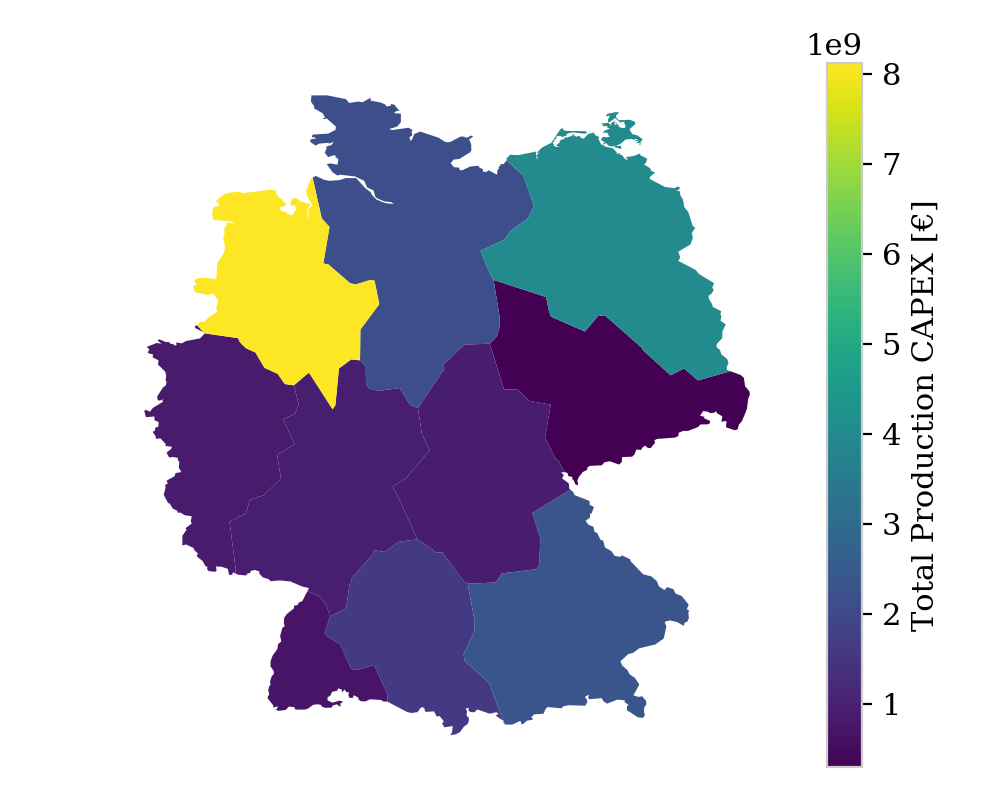
\includegraphics[width=\linewidth]{de50bf/maps_price_ptpf_net/one_port_investment_cost_total}
%         \subcaption{All production and storage technologies}
%         \label{fig:total_capex}
%     \end{subfigure}
%     \begin{subfigure}[c]{.49\linewidth}
%         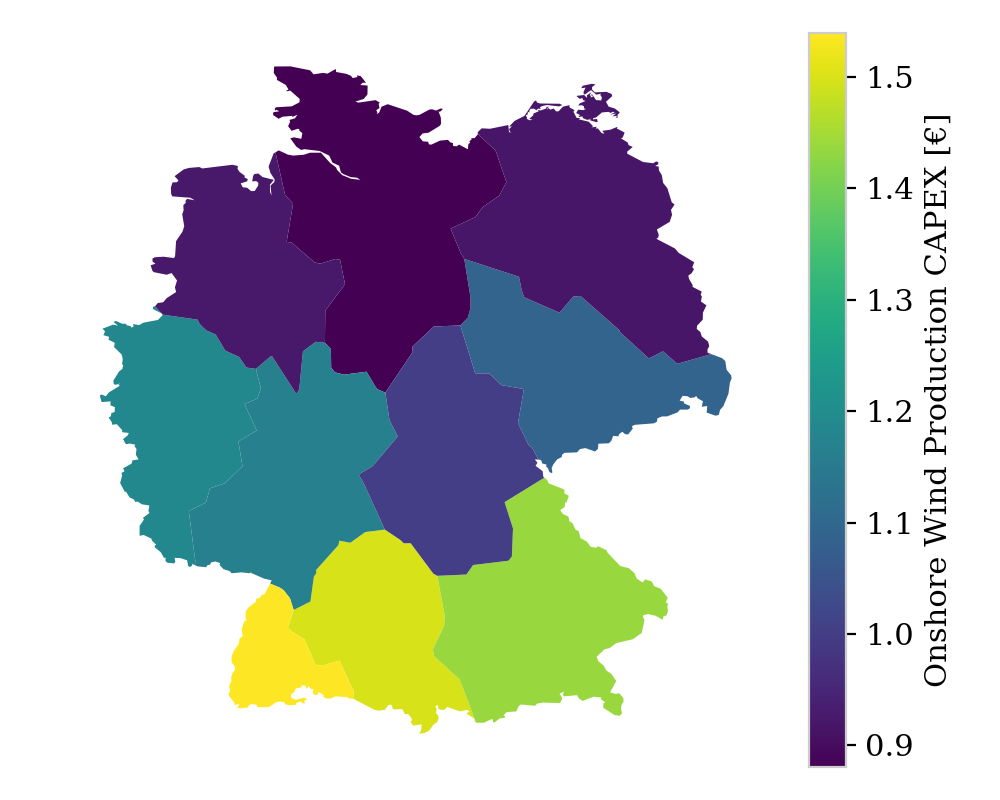
\includegraphics[width=\linewidth]{de50bf/maps_price_ptpf_net/by_carrier/onwind_one_port_investment_cost}
%         \subcaption{Onshore Wind}
%         \label{fig:onshore_capex}
%     \end{subfigure}
%     \begin{subfigure}[c]{.49\linewidth}
%         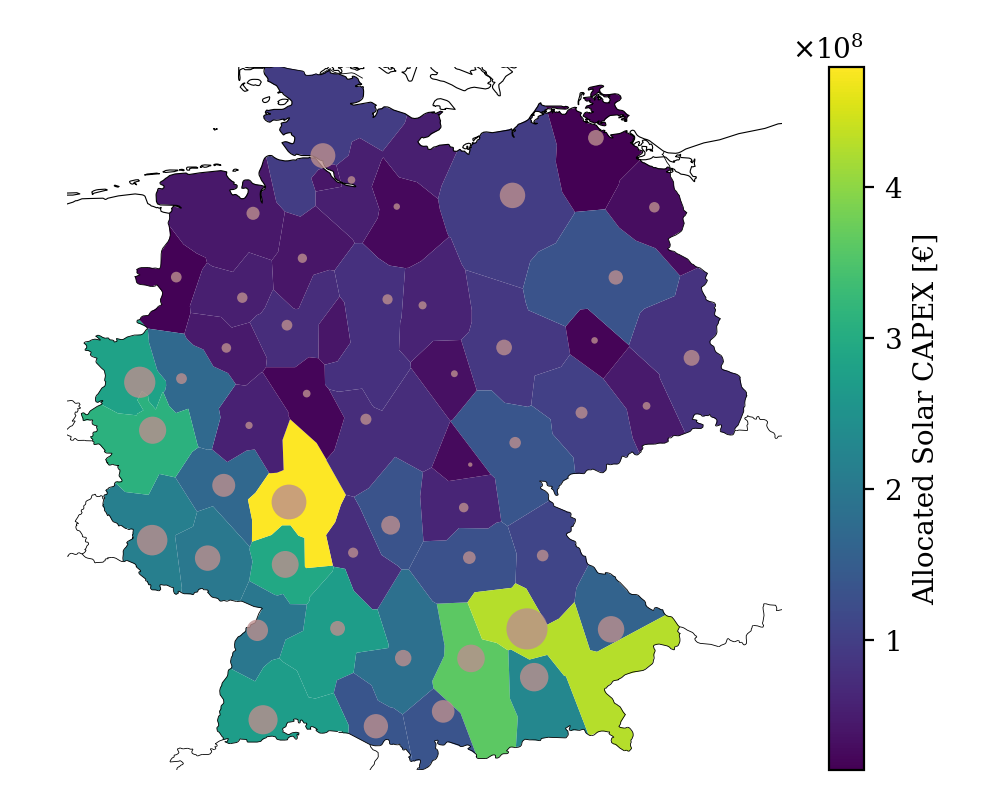
\includegraphics[width=\linewidth]{de50bf/maps_price_ptpf_net/by_carrier/solar_one_port_investment_cost}
%         \subcaption{Solar}
%         \label{fig:solar_capex}
%     \end{subfigure}
%     \begin{subfigure}[c]{.49\linewidth}
%         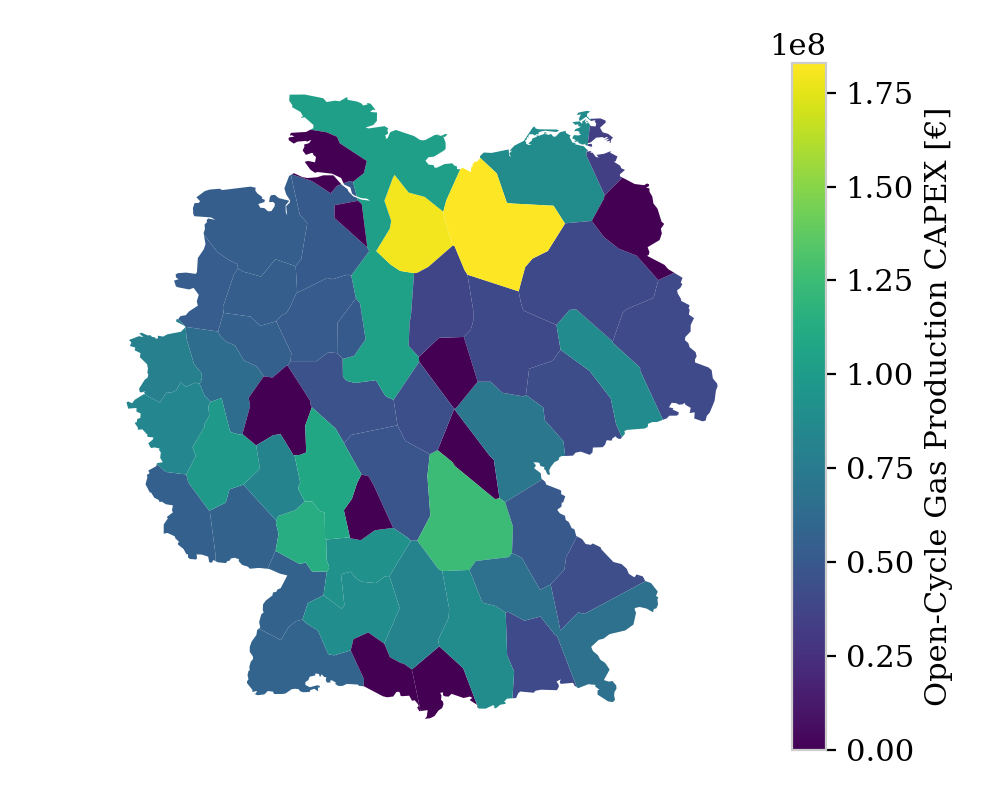
\includegraphics[width=\linewidth]{de50bf/maps_price_ptpf_net/by_carrier/OCGT_one_port_investment_cost}
%         \subcaption{OCGT}
%         \label{fig:ocgt_capex}
%     \end{subfigure}
%     \caption{Average \textbf{CAPEX allocation} per MWh, $\sum_t \allocatecapex / \sum_t \demand$  for all production and storage assets (a), onshore wind (b), solar (c) and OCGT (d). Average allocated CAPEX per MWh within the regions are indicated by the color, the revenue per production asset is given by the size of the circles at the corresponding bus.}
%     \label{fig:capex_price}
% \end{figure*}




% \begin{figure}
%     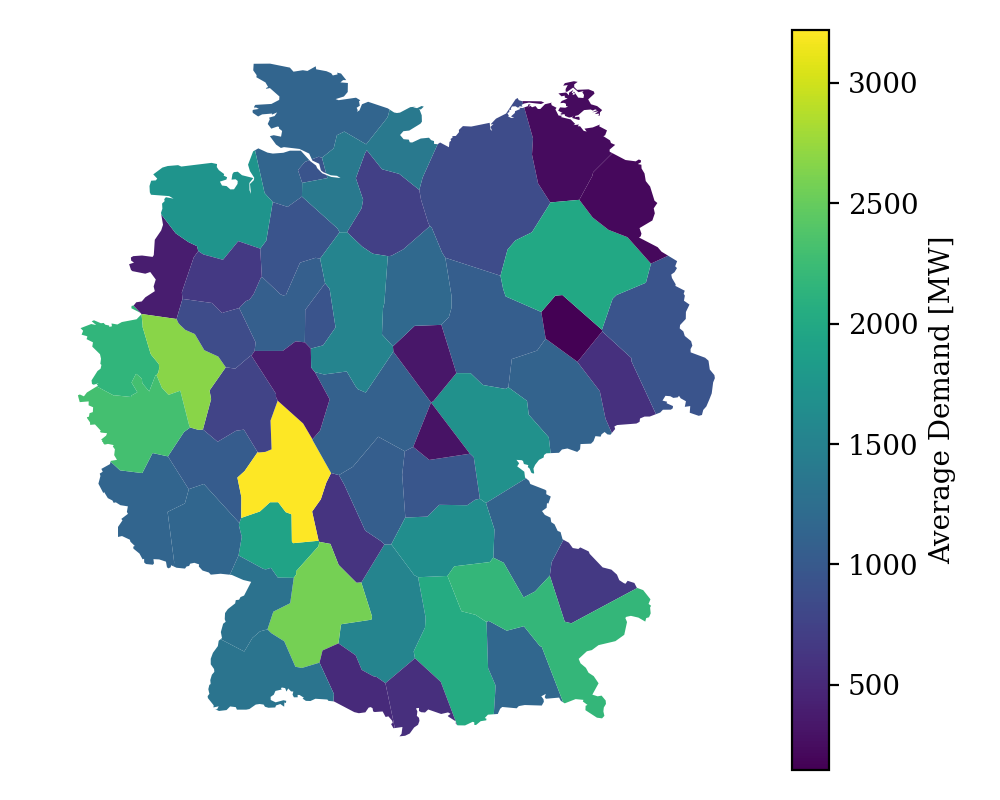
\includegraphics[width=\linewidth]{de50bf/average_demand}
%     \caption{Average demand, $\sum_t \demand/T$ per regions. The regions with high population densities and larger areas reveal a higher demand.}
%     \label{fig:average_demand}
% \end{figure}


% \begin{figure}
%     \includegraphics[width=\linewidth]{de50bf/power_mix_ptpf_net}
%     \caption{Average power mix per region calculated by Average Participation. Coastal regions are mainly supplied by local offshore and onshore wind farms. Their strong power injections additionally penetrate the network up to the southern border. In the middle and South, the supply is dominated by a combination of OCGT and solar power.}
%     \label{fig:power_mix}
% \end{figure}

% \begin{figure}
%     \vspace{2cm}
%     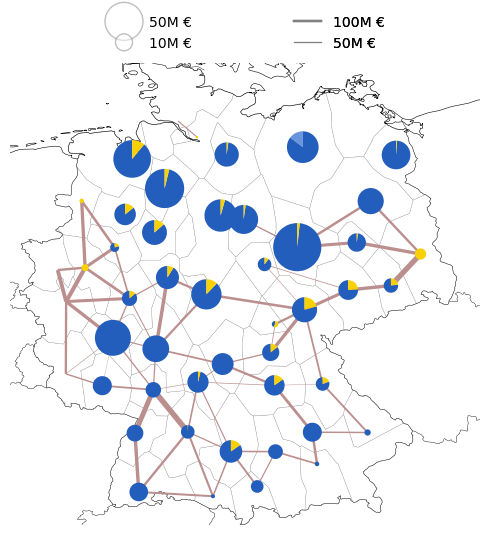
\includegraphics[width=\linewidth]{de50bf/subsidy}
%     \caption{Total costs for subsidy $\subsidycost$ resulting from lower capacity expansion bounds (brownfield constraints). The figure shows the built infrastructure that does not gain back its CAPEX from its market revenue, but is only built due to lower capacity limits.}
%     \label{fig:subsidy}
% \end{figure}


% \begin{figure*}
%     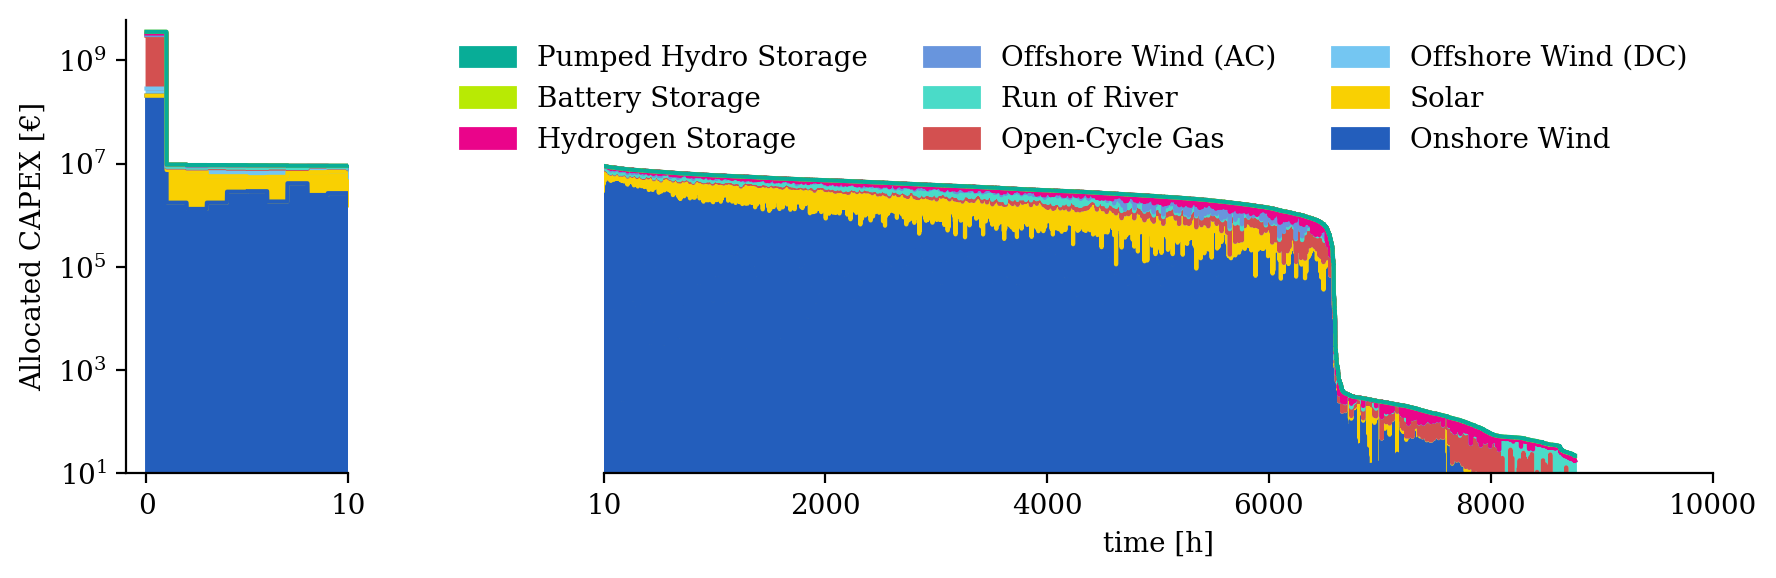
\includegraphics[width=\linewidth]{de50bf/capex_duration_curve}
%     \caption{Duration curve of the CAPEX allocation for production and storage technologies. Hours are sorted by the total amount of allocated expenditure. With 2.7 bn~\euro\, the first value pushes investments extraordinarily high. Due to low renewable potentials, it is dominated by CAPEX for OCGT which receives 92\% of the payments. This hour alone occasions about the half of all OCGT CAPEX. \Cref{fig:capex_duration_curve} gives a detailed picture of the operational state at this time-step. The following 7000 time-steps are dominated by revenues for onshore wind and reveal a rather even distribution. In hours of low CAPEX allocation (after the second drop) spending for OCGT start to increase again. These time-steps however play a minor role.}
%     \label{fig:capex_duration_curve}
% \end{figure*}

% \begin{figure}
%     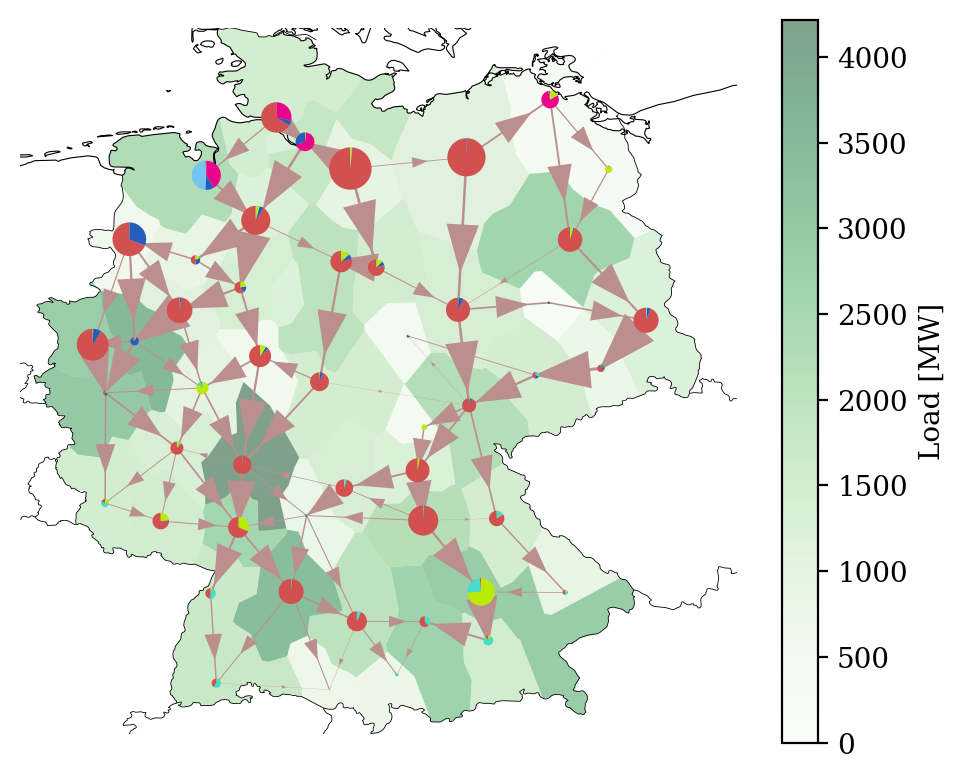
\includegraphics[width=\linewidth]{de50bf/operation_high_expenditure}
%     \caption{Production, flow and consumption in the system at the hour with the highest allocated expenditures. The size of the circles are proportional to the power production at a node. Size of arrows are proportional to the flow on the transmission line. The depicted hour corresponds to the first value in the duration curve in \cref{fig:capex_duration_curve}.}
%     \label{fig:operation_high_expenditure}
% \end{figure}


% \begin{figure}
%     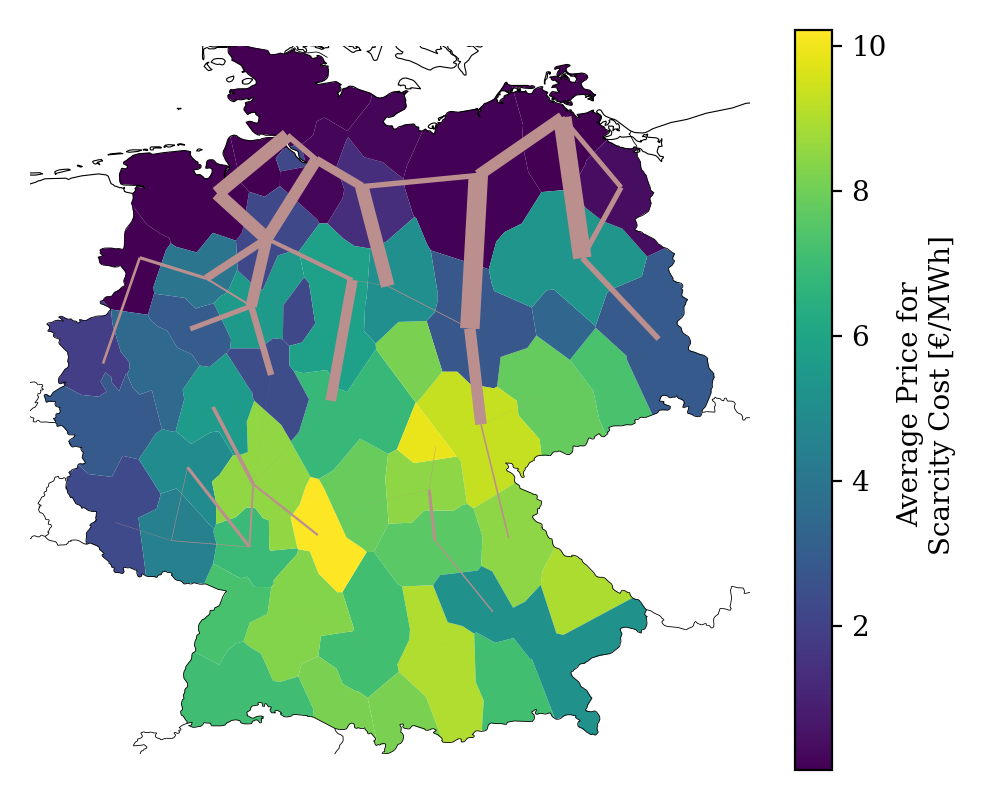
\includegraphics[width=\linewidth]{de50bf/maps_scarcity_price_ptpf_net/branch_scarcity_cost_total}
%     \caption{Average \textbf{allocated transmission scarcity cost} per consumed MWh, $\sum_t \scarcitycost_{n \rightarrow \ell, t} / \sum_t \demand $. This scarcity cost results from the upper transmission expansion limit of 25\%. The costs are indicated by the regional color.  The lines are drawn in proportion to revenue dedicated to scarcity cost. }
%     \label{fig:branch_scarcity_price}
% \end{figure}




% \begin{figure*}
%     \centering
%     \begin{subfigure}[c]{.49\linewidth}
%         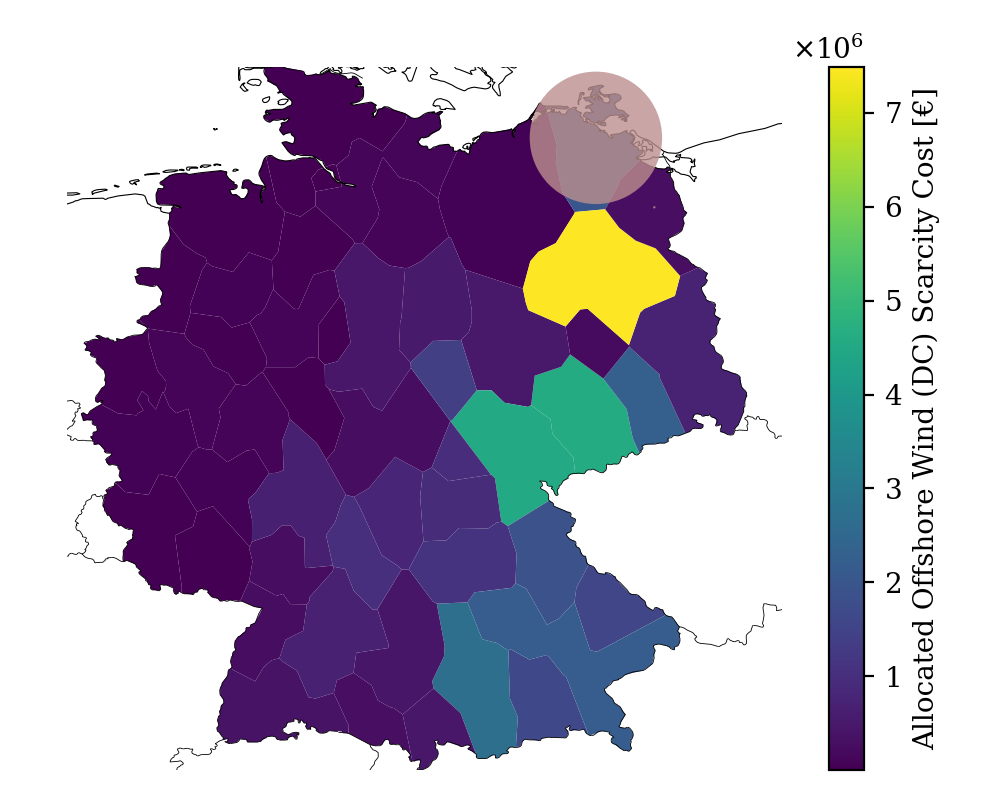
\includegraphics[width=\linewidth]{de50bf/maps_scarcity_price_ptpf_net/by_carrier/offwind-dc_generator_scarcity_cost}
%         \subcaption{Offshore Wind}
%         \label{fig:offwind-dc_generator_scarcity_cost}
%     \end{subfigure}
%     \begin{subfigure}[c]{.49\linewidth}
%         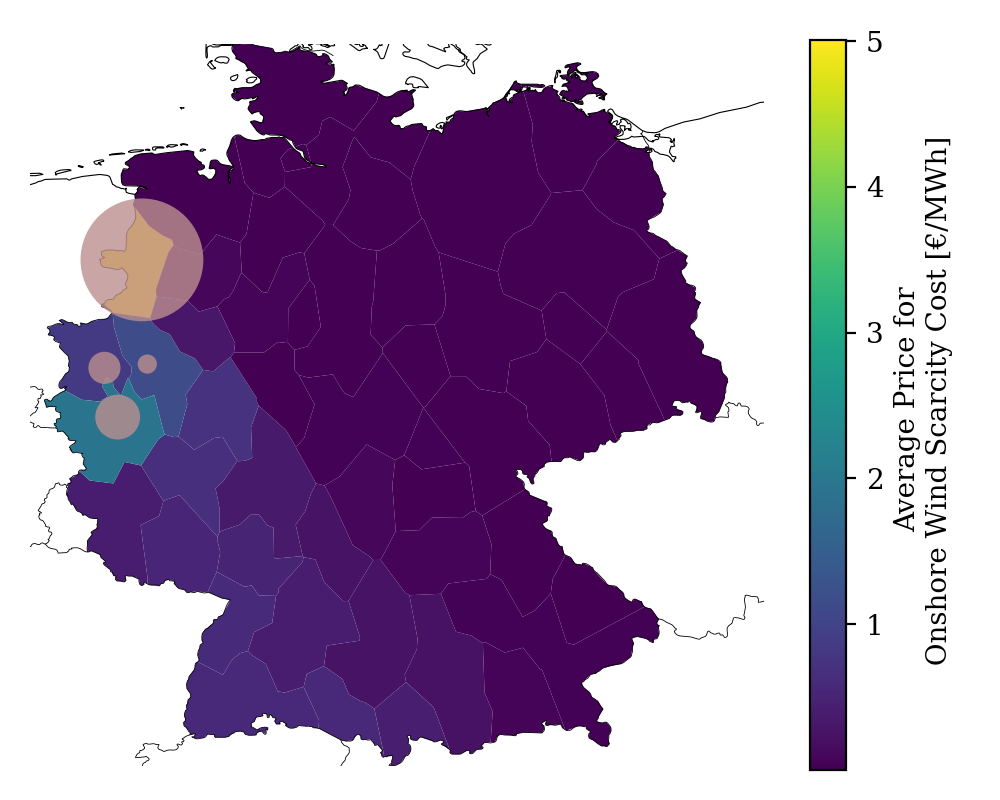
\includegraphics[width=\linewidth]{de50bf/maps_scarcity_price_ptpf_net/by_carrier/onwind_generator_scarcity_cost}
%         \subcaption{Onshore Wind}
%         \label{fig:onwind_generator_scarcity_cost}
%     \end{subfigure}
%     \begin{subfigure}[c]{.49\linewidth}
%         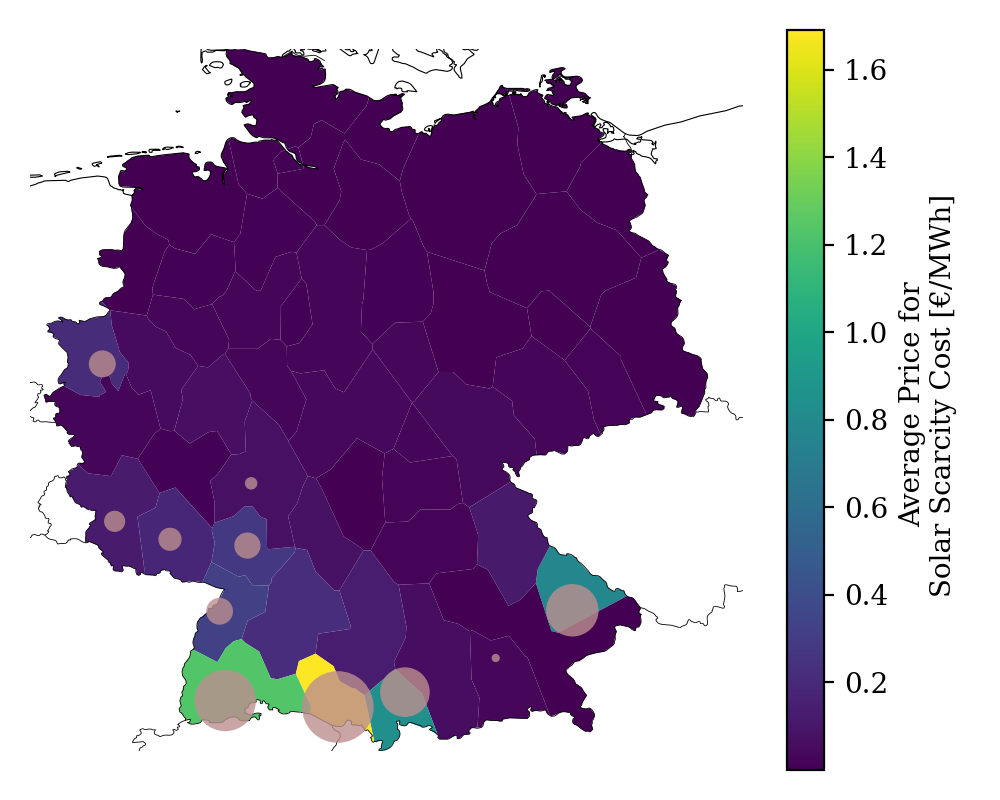
\includegraphics[width=\linewidth]{de50bf/maps_scarcity_price_ptpf_net/by_carrier/solar_generator_scarcity_cost}
%         \subcaption{Solar}
%         \label{fig:solar_generator_scarcity_cost}
%     \end{subfigure}
%     \begin{subfigure}[c]{.49\linewidth}
%         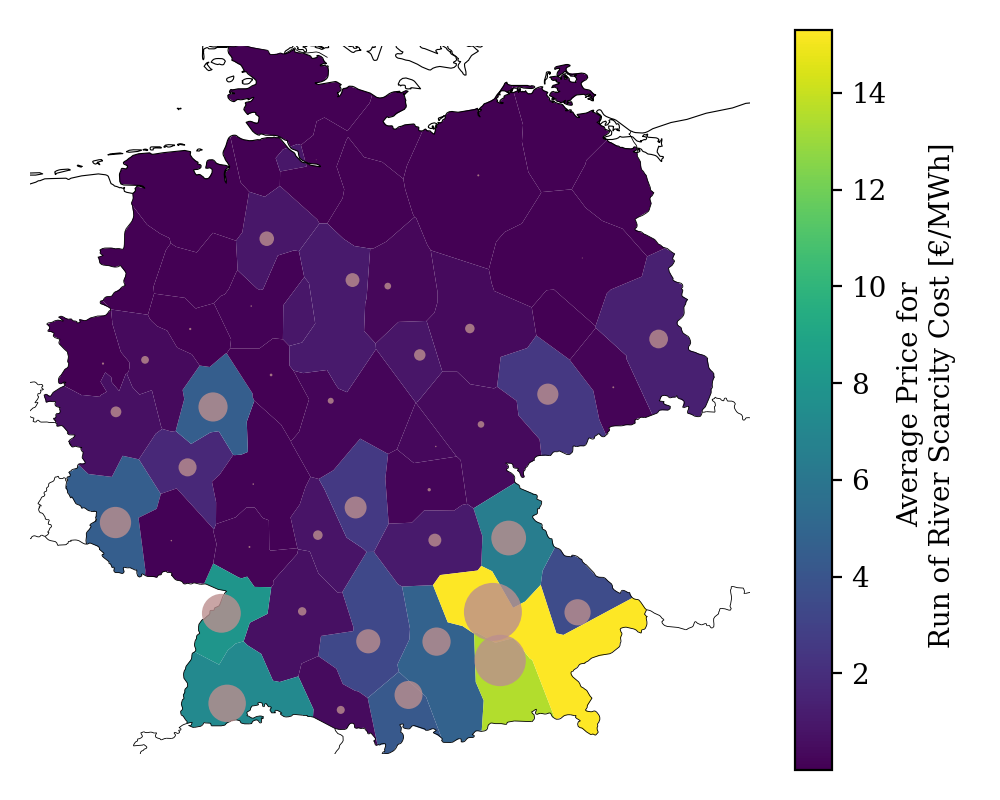
\includegraphics[width=\linewidth]{de50bf/maps_scarcity_price_ptpf_net/by_carrier/ror_generator_scarcity_cost}
%         \subcaption{Run-of-River}
%         \label{fig:ror_generator_scarcity_cost}
%     \end{subfigure}
%     \caption{Average \textbf{allocated scarcity cost} per consumed MWh, $\sum_t \allocatescarcitycost / \sum_t \demand$. These cost result from land use restrictions for offshore wind, onshore wind,  solar, run-of-river. The cost per MWh are indicated by the color of a region. The revenue per production asset is given by the size of the circle at the corresponding bus.}
%     \label{fig:scarcity_price}
% \end{figure*}





\clearpage
\printbibliography





\end{document}
